\documentclass[a4paper]{report}
%\documentclass[a4paper,twoside,openright]{report}
\usepackage[utf8]{inputenc}
\usepackage[T1]{fontenc}
\usepackage[ngerman,english]{babel}
\usepackage{titlesec}
\usepackage{subfigure}
\usepackage{graphicx}
\usepackage{parskip}
\usepackage{lmodern}
\usepackage{adjustbox}
\usepackage{tikz}
\usepackage{amsmath}
\usepackage{caption}
\usepackage{cite}
\usepackage{listings}
\usepackage{algorithm}
\usepackage{algorithmic}
\usepackage{pdflscape}
\usepackage[hidelinks]{hyperref}
\usetikzlibrary{arrows,shapes,fit,positioning}
\usetikzlibrary{decorations.pathmorphing}
\usetikzlibrary{decorations.markings}
\graphicspath{{figures/}}

\lstset{basicstyle=\footnotesize\ttfamily,breaklines=true}
\lstset{framextopmargin=50pt,frame=bottomline}
\lstset{
    captionpos=b,
    numbers=left,
    stepnumber=1,
    tabsize=1,
}

\titleformat{\chapter}[display]
{\normalfont\huge\bfseries}{\chaptertitlename\ \thechapter}{20pt}{\Huge}

% configure autoref
\addto\extrasenglish{
	\def\chapterautorefname{Chapter}
	\def\subsectionautorefname{Subsection}
	\def\sectionautorefname{Section}
}

% this alters "before" spacing (the second length argument) to 0
\titlespacing*{\chapter}{0pt}{-50pt}{20pt}

\author{}
\date{\today}
\begin{document}
\pagestyle{empty}
\begin{titlepage}
\begin{center}
  % Upper part of the page  
	
\includegraphics[width=10cm,clip,trim=0 0 0 0\textwidth]{rptu}\\[2cm]
	% {
	% 	\linespread{1.5}\selectfont
	% 	\textsc{\LARGE Rheinland-Pfälzische Technische Universität Kaiserslautern-Landau}\\[0.5cm]
	% }
  \textsc{\large Fachbereich Informatik}\\[1.5cm]
	\vfill
  \textsc{\Large Bachelor's Thesis}\\[0.5cm]
{
  \linespread{1.0}\selectfont
{\LARGE   \textsc{Design and Implementation of a Distributed Dataset Search Infrastructure}\\[2cm]}
}

  { \Large
  Author:\\
	Nhat Anh Pham\\[2cm]
  {\small submitted on: \\
  \today}
  }\\[1cm]

  Supervisor\\
Prof. Dr.-Ing. Sebastian Michel\\[2cm]

  Reviewers\\
.....\\
  Prof. Dr.-Ing. Sebastian Michel\\

  
\end{center}
\end{titlepage}

%
\cleardoublepage


\begin{abstract}
In a distributed environment, where servers communicate via wireless networks and each server hosts a collection of datasets, finding relevant information across servers can be challenging. If a user from one server wants to identify datasets from other servers that can be joined or unioned with their own, traditional search systems would fall short because they don't consider the attributes of the datasets. Moreover, it is infeasible to transmit entire datasets across the network to find potential matches due to their large size. In this thesis, we introduce a lookup infrastructure for relational datasets that allow users to query with a dataset and receive results from other servers that are joinable/unionable with the query. Our system utilizes different measures to create compact summaries the datasets, which is significantly smaller in size than the original data. The summaries are then used to compare datasets for similarities. Through empirical evaluation, we show that the system is efficient in finding related datasets and can provide comparable response time to state-of-the-art dataset search systems, while minimizing the network traffic.
\end{abstract}

\cleardoublepage

\selectlanguage{ngerman}
\begin{abstract}
In einer verteilten Umgebung, in der Server über drahtlose Netzwerke kommunizieren und jeder Server eine Sammlung von Datensätzen hostet, kann das Finden relevanter Informationen über Server hinweg eine Herausforderung darstellen. Wenn ein Benutzer von einem Server Datensätze von anderen Servern identifizieren möchte, die mit seinen eigenen zusammengeführt oder vereinigt werden können, stoßen herkömmliche Suchsysteme an ihre Grenzen, da sie die Attribute der Datensätze nicht berücksichtigen. Darüber hinaus ist es aufgrund der großen Datenmengen nicht praktikabel, ganze Datensätze über das Netzwerk zu übertragen, um potenzielle Matches zu finden. In dieser Arbeit stellen wir eine Lookup-Infrastruktur für relationale Datensätze vor, die es Benutzern ermöglicht, mit einem Datensatz zu suchen und Ergebnisse von anderen Servern zu erhalten, die mit der Anfrage joinbar oder unionbar sind. Unser System nutzt verschiedene Maßnahmen, um kompakte Zusammenfassungen der Datensätze zu erstellen, die deutlich kleiner sind als die Originaldaten. Diese Zusammenfassungen werden dann verwendet, um Datensätze auf Ähnlichkeiten zu vergleichen. Durch empirische Evaluierung zeigen wir, dass das System effizient verwandte Datensätze findet und eine vergleichbare Reaktionszeit zu modernen Datensatz-Suchsystemen bietet, während der Netzwerkverkehr minimiert wird.
\end{abstract}
\selectlanguage{english}

\tableofcontents
\thispagestyle{empty}
\listoffigures
\thispagestyle{empty}
\begingroup
\thispagestyle{empty}
\let\clearpage\relax
\vspace{3cm}
\listofalgorithms
\let\clearpage\relax
\vspace{3cm}
\listoftables
\endgroup
\thispagestyle{empty}


%%% 
%%% Add your inputs here
%%%

% !TEX root =  main.tex



\chapter{Introduction}
\label{chap:introduction}
\pagestyle{plain}
\setcounter{page}{1}

Lorem ipsum





% !TEX root =  main.tex



\chapter{Background Knowledge}
\label{chap:background}
\pagestyle{plain}

In this chapter, we give context on the terminologies, definitions and algorithms employed in our system.

\section{Schema Matching}\label{schemaMatching}
Schema matching is the task of finding semantic correspondence between two schemas, where a schema is defined as a set of elements connected by some structure \cite{schemaMatching}. It plays a critical role in data integration and translation applications. An use case example is the integration of a real estate schema and a property tax schema, where each schema may have structural and terminological differences, but occur in the same real-world domain and thus can be unified under the same schema. In the case of relational data, schema matching techniques can be used to determine the joinability and unionability between attributes of two tables \cite{valentine}. Schema matching techniques for relational data work on attributes/columns of tables and can be roughly classified into two categories: schema-based and instance-based:

\begin{description}
    \item[Schema-based] These types of matchers only consider the schema-level information of a dataset such as table name, attribute names, description, data type, constraints, etc \cite{cupid}. The similarity of the information can be calculated by e.g. how much the attribute name syntactically or semantically overlap, is the data type similar (short and int or text and varchar).
    \item[Instance-based] When schema-level information is limited, the instances of an attribute can provide correct interpretation of schema information. Examples include the similarity in how the instances of two attributes overlap, or how the format patterns look like (money-related instances contain a currency symbol, whereas a zip code does not).
\end{description}

Matching process usually involves calculating the degree of similarity by a normalized numeric value in the range 0 to 1. It is also possible to combine different matching techniques together, then an algorithm is applied to aggregate the score of different techniques to one single score that is used to rank the results \cite{coma}. In our implementation, we will follow this hybrid strategy.

\section{Similarity Metrics}

\subsection{Levenshtein distance similarity}

In order to capture the syntactic relatedness between two words \(s\) and \(t\), we use the Levenshtein edit distance. The Levenshtein distance between two words is the minimum required number of insertions, deletions or substitutions of a character to transform one word into another \cite{levenshtein}. Since this metric measures distance, we convert it into a similarity metric by dividing the distance with the length of the longest word, normalizing it to the range 0 and 1, and then subtract it from 1 to get a similarity score:

\[sim_{levenshtein} = 1 - \frac{dist(s, t)}{max(s, t)}\]

\subsection{WordNet Similarity}\label{wordnet}

In order to capture the semantic relatedness between two words, we use the machine-readable lexical database WordNet \cite{wordnet}, which contains English words grouped into sets of synonyms (synsets) and structured in a hierarchical is-a relation. One algorithm that can be used to calculate the similarity of two words \(s\) and \(t\) is the Wu-Palmer algorithm \cite{wuPalmer}, which considers the depths of two synsets in the Wordnet hierarchy as well as the depth of the least common subsumer (LCS) i.e. the most specific concept that is the ancestor of both \(s\) and \(t\):

\[sim_{wordnet}(s, t) = 2 \cdot \frac{depth(LCS)}{(depth(s) + depth(t))}\]

To extend the similarity of two words to two sets of words / sentences \(q_i\) and \(q_j\), we use an equation similar to ones from \cite{wordnetSim} and \cite{cupid}:

\[score(q_i, q_j) = \frac{\Sigma_{s \in q_i} sim_m(s, q_j) +\Sigma_{s \in q_j} sim_m(s, q_i)}{|q_i| + |q_j|}\]

where \(sim_m(s, q_j\) is the similarity score of s and the word in \(q_j\) that has the highest similarity score. If a word does not exist in the dictionary, we fall back to Levenshtein distance similarity for the calculation.

\subsection{Jaccard Similarity}\label{js}

The Jaccard similarity/coefficient is a metric used to calculate the similarity of two sets  \cite{miningOfMassiveDatasets}. Given two sets \(A\) and \(B\), the Jaccard coefficient \(J(A, B)\) of the two sets is defined by the ratio between the size of the intersection to the size of the union:

\[
J(A, B) = \frac{|A \cap B|}{|A \cup B|}
\]

For example, if \(A = \{1, 2, 3\}\) and \(B = \{2, 3, 5\}\), then \(J(A, B) = \frac{1}{2}\). The value of Jaccard coefficient ranges from 0 to 1. In \cite{tusZhu}, the authors show that a high Jaccard coefficient value between sets suggests a high probability that the elements of the sets are drawn from the same domain. Therefore, we can utilize this measure to find unionable columns for a given column of a dataset.

\subsection{Set Containment}\label{jc}

One problem with Jaccard coefficient is that the measure is symmetric. In the case where sets are of vastly different sizes, the measure is biased to sets with smaller sizes \cite{lshEnsemble}. For example, consider the query set:

\begin{itemize}
    \item \(Query\) = \{Ontario, Toronto\}
\end{itemize}

and the two sets:

\begin{itemize}
    \item \(Provinces\) = \{Alberta, Ontario, Manitoba\}
    \item \(Locations\) = \{Illinois, Chicago, New York City, New York, Nova Scotia, Halifax, California, San Francisco, Seattle, Washington, Ontario, Toronto\}
\end{itemize}

We see that while the \(Locations\) set contain all the elements of the \(Query\) set, their Jaccard similarity is only 0.083, while the similarity between \(Query\) and \(Provinces\) is at 0.25, indicating a higher degree of relatedness despite \(Provinces\) containing only one similar element with \(Query\). Due to this reason, there is another asymmetric measure used in the literature for comparing set similarity called set containment.

Given two sets \(A\) and \(B\), the set containment of \(A\) in \(B\) is defined as:

\[
J_C(A, B) = \frac{|A \cap B|}{|A|}
\]

and vice versa for the containment of \(B\) in \(A\):

\[
J_C(B, A) = \frac{|A \cap B|}{|B|}
\]

Using set containment, we see that \(J_C(Q, Provinces)\) is 0.5, while \(J_C(Q, Locations)\) is now 1.0. This measure is proven to be useful in identifying primary-key/foreign-key relationships, which enables the process of finding joinable datasets \cite{lazo}.

\section{Q-gram}

Another way to measure the syntactic relatedness of two words beside using Levenshtein distance similarity, is by comparing their q-grams sets. A q-gram (or n-gram) of a string is simply a substring of length q \cite{qgram}. The set of q-grams of a string is then constructed by finding all q-grams within that string. We utilize the Jaccard coefficient mentioned above to calculate the similarity of the q-grams sets. For example, to compare "house" and "horse" with a q value of 2:

\begin{itemize}
    \item 2-grams of "house": \(s = \{ho, ou, us, se\}\)
    \item 2-grams of "horse": \(t = \{ho, or, rs, se\}\), therefore:
\end{itemize}

\[sim_{qgram}(house, horse) = J(s,t) = \frac{1}{3}\]

The advantage of this measure compared to Levenshtein distance similarity is, they can be efficiently calculated using locality sensitive hashing, which is explained in section \ref{lsh}.

\section{MinHash Sketch}

When a set size goes to the degree of thousands of elements or higher, calculating the Jaccard coefficient/containment of two sets can become computationally very expensive. Instead, we transform the sets into smaller, fixed-size representations called "sketches" and calculate the similarity measures using only these sketches \cite{miningOfMassiveDatasets}. One of these types of sketches is called MinHash.

The core idea behind MinHash is to apply a hash function to the elements of a set, simulating a random permutation, and then store the minimum hash value observed. By doing this multiple times with different hash functions, we create a set of minimum values that serves as a compact representation of the original set. The interesting property of MinHash is that, the probability of 2 sets having the same minimum hash value when applied the same hash function is directly related to the Jaccard coefficient between two sets:

\[Pr[h_{min}(A) = h_{min}(B)] = \frac{|A \cap B|}{|A \cup B|} = J(A, B)\]

Thus, by using \(k\) multiple hash functions, the Jaccard coefficient can be estimated as:

\[J(A, B) = \frac{1}{k} \cdot \Sigma \; \mathbf{1}((h^i_{min}(A) = h^i_{min}(B))\]

Where the function \(\mathbf{1}\) returns 1 if the condition inside the argument is true and 0 otherwise.

\section{Locality Sensitive Hashing} \label{lsh}

While MinHash allows us to efficiently calculate similarity of sets, it remains a challenge to find the pairs with greatest similarity among large collection of sets, since we would need to perform up to pairwise calculations of all pairs of sets to get the correct result. However, for our task we would want only the most similar pairs or pairs that are above some similarity threshold. Therefore, we accept a slight loss in accuracy and use approximate methods to focus our attention only on pairs that are likely to be similar, without investigating every pair. One such method is locality sensitive hashing (LSH), which is widely used in data discovery tasks due to its exploratory and imprecise nature. \cite{miningOfMassiveDatasets, lazo}

The general idea of LSH is to use a locality sensitive hash function to hash items into buckets, where the amount of buckets is significantly smaller than the universe of the possible input items. Locality sensitive hash functions are functions which map inputs that are similar to the same hash value with high probability, while minimizing that probability for inputs that are dissimilar \cite{lshDefinition}. If we use these hash functions to map elements in the buckets, similar items would fall into the same buckets with high probability. Thus, in order to find similar items with our input, we need only to check the similarity of the items in the bucket that our input falls into. 

In literature, the way a MinHash sketch in hashed into a LSH index is by first diving it into \(b\) bands of equal length, then hash each of these bands into individual bucket array. Two sketches are similar if in any band, there is a bucket collision ( figure \ref{fig:lsh}). The use of LSH functions mean the more similar two sketches are, the higher the probability they will be identical in at least one band, making them candidate pairs. This banding strategy thus enhances the likelihood of detecting similar columns while minimizing accidental collisions for dissimilar pairs.

\begin{figure}[h]
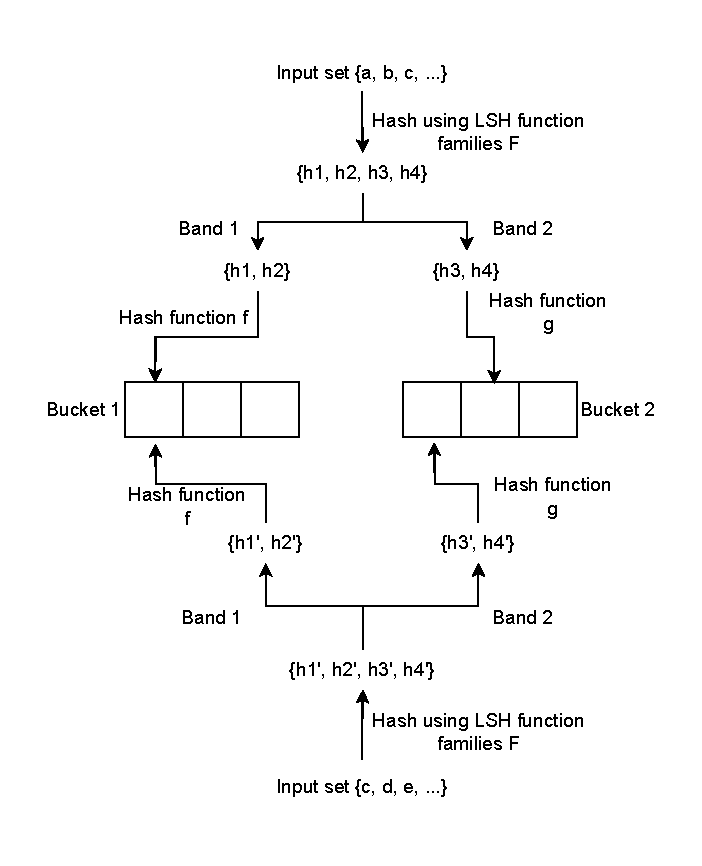
\includegraphics[scale=0.8]{lsh.pdf}
\centering
\caption{Example of the LSH banding technique. The two sketches collide in bucket 1, hence a match}
\label{fig:lsh}
\end{figure}

\section{REST API}

Representational State Transfer (REST) is a term coined by Fielder in his PhD dissertation \cite{rest}. It is a software architectural style that defines a set of constraints on how the components of a distributed hypermedia system like in Web should communicate with each other. Rest API is an application programming interface (API) that adheres to the constraints of REST architectural style. While there are six constraints that Fielder introduced in his work, the three most important constraints for our work are:

\begin{itemize}
    \item \textbf{Uniform interface}: REST components communicate with each other via representation or abstraction of resources but still need to contain enough information to manipulate the underlying resources. They are identifiable using Unique Resource Identifiers (URIs).
    \item \textbf{Client-server decoupling}: Client and server are independent of each other. Communications between client and server happen between an interface, i.e. the URI of a resource.
    \item \textbf{Statelessness}: Each request from client to server must contain all the information required to process the request, without utilizing additional server context.
\end{itemize}

Overall, these constraints allow a system to have better performance thanks to its flexibility and scalability. In practice, REST APIs work through HTTP connections, which fit the constraints of REST perfectly. A REST API request contains the following component:

\begin{itemize}
    \item \textbf{Endpoint}: The URI where the requested resource can be retrieved. For instance, the URI for a HTTP request is an Unified Resource Locator (URL): \nolinkurl{https://song.com/trackID/1}
    \item \textbf{Method}: The HTTP method that is used to operate on the resources. The common methods are GET (retrieve a resource), POST (Create a new resource), PUT (update existing resource) and DELETE (remove a resource).
    \item \textbf{Headers}: Provide metadata-level information about the request like the content type or its encoding.
    \item \textbf{Parameters}: Additional information that is appended to the URL to specify server's action in a more detailed way.
    \item \textbf{Request body}: The data, which is a representation of resource that is sent to the server. It is often formatted in JSON.
\end{itemize}

Upon receiving a request, the server responds with a HTTP response, containing the response metadata, a status code to indicate whether the request was successful or not and the resource representation itself in the body. Due to the nature of our system working in a distributed environment, REST APIs are employed to facilitate communication between the components.
% !TEX root =  main.tex



\chapter{Related Work}
\label{chap:relatedwork}
\pagestyle{plain}

\section{Valentine}

In Valentine \cite{valentine}, Koutras et al. presented an experiment suite designed to evaluate various schema matching methods for dataset discovery, as these tasks rely heavily on schema matching to find joinable and unionable datasets. The schema matching methods they evaluated were group into six categories:

\begin{itemize}
    \item \textbf{Attribute overlap matcher}: Two columns are related if their attribute names have syntactic overlap above a predefined threshold.
    \item \textbf{Value overlap matcher}: Two columns are related when their value sets/instances have high degree of overlap.
    \item \textbf{Semantic overlap matcher}: Two columns are related when they have significant overlap in their labels or domain, according to some source of external knowledge.
    \item \textbf{Data type matcher}: Matches columns that have similar data types.
    \item \textbf{Distribution matcher}: Matches columns based on how similar the distributions of the values are.
    \item \textbf{Embeddings matcher}: Two columns are related if they are highly similar in the embeddings of the values, which are derived from an existing pre-trained model on natural language corpora.
\end{itemize}

The methods are then ranked across four relatedness scenario:

\begin{itemize}
    \item \textbf{Joinable relations}: There exists at least one pair of attributes coming from each relation on which a join can be executed.
    \item \textbf{Semantically-joinable relations}: There exists at least one pair of attributes coming from each relation that is semantically (must not syntactically) related and on which a semantic join can be executed. Such joins are called "fuzzy".
    \item \textbf{Unionable relations}: Two relations have the same arity and there exists a 1-1 mapping, denoting semantic equivalence between their attribute sets.
    \item \textbf{View-unionable relations}: There exists a view of each relation such that the two views are unionable.
\end{itemize}

For each scenario, a match is defined as a pair of attributes from two different relations. The matches are ranked in descending order according to their similarity scores. The notions introduced in Valentine, along with the datasets they used, serve as a baseline for how we implement and evaluate our systems.

\section{D3L}

In the paper "Dataset Discovery in Data Lakes" by Bogatu et al., the authors introduced  \(D^3L\), a dataset discovery framework that utilizes LSH indexes to to efficiently determine the relatedness (joinability and unionability) between attributes of datasets in data lake. The similarity measures that are inserted into the indexes are:

\begin{itemize}
    \item Attribute name: Calculate similarity based on the n-gram sets of the attribute name.
    \item Attribute values overlap: Calculate similarity based on how much the attributes' values overlap.
    \item Word-embedding: Calculate similarity based on semantic relatedness of the attribute' values by representing words as multi-dimensional vectors.
    \item Format representation: Calculate similarity based on the regular representation patterns of the attributes' values
    \item Domain distribution: For numerical attributes, calculate similarity based on how close the values are in their distribution.
\end{itemize}

The values of each measurements are combined into a single relatedness by calculating their weighted sum, where the weights are obtained using machine learning. Our work is inspired by the use of LSH indexes for similarity calculation and the weighted sum used to calculate the final score. Similar to \(D^3L\), we will also be using attribute name, attribute values overlap and the format representation as our measure of similarity. We choose not to use word-embedding similarity due to low precision and recall results evaluated in the paper as well as in \cite{valentine}. The distribution similarity is also not used due to it not being indexable into LSH index and require the reading of all attribute instances, which is not suitable when we are working in a distributed environment. 

\section{Lazo}\label{lazo}

In \cite{lazo} by Fernandez et al., the authors proposed Lazo, a method that efficiently estimate both Jaccard similarity and set containment of sets by redefining Jaccard similarity to include set cardinality, which allows for independent estimation of intersection and union of sets. At the beginning of the paper, they also mentioned some problems with traditional LSH index that makes it difficult to be directly applied to the data discovery problem:

\begin{itemize}
    \item LSH cannot estimate set containment since that requires estimating the size of the intersection, which is difficult to do with LSH. On the other hand, LSH methods that do support set containment do not support incremental indexing, which means items can no longer be hashed to the index after being queried. This makes those methods unable to work in the context of dataset discovery/schema matching, where datasets are always changing or there are new data arriving.
    \item The indexes do not return a similarity score. As mentioned in \ref{lsh}, the LSH index only return candidates that are hashed into the same buckets. In order to obtain a score, we would either have to manually perform the calculation, or use multiple indexes with different similarity threshold and query them all, both of which are costly and inefficient.
\end{itemize}

As a result, they presented Lazo index, a modified LSH index that allows query using arbitrary input thresholds and returns a set of candidates along with their corresponding Jaccard similarity and set containment. Evaluation of their approach shows that the Lazo index significantly enhances indexing speed and provides 2-10x faster query speed compared to traditional LSH indexes. Additionally, their method outperforms other LSH methods that support set containment estimation, providing higher estimation quality. Testing on large datasets also showed that the overhead of applying the Lazo method is negligible in practice, making it suitable for data discovery scenarios. In fact, Lazo has already been used in some recent novel dataset search systems \cite{aurum, auctus}. In our implementation, we will also be using Lazo and Lazo index to efficiently query similarities between datasets.



% !TEX root =  main.tex



\chapter{System Overview}
\label{chap:overview}
\pagestyle{plain}

This chapter presents the measures of similarity used in our system as well as giving a high-level introduction to the system's architecture, how it is set up in a distributed environment, how user can use it to query for similar datasets.

\section{Measures of similarity}\label{simMeasures}

As mentioned in section \ref{schemaMatching}, the task of similarity search is comparable to the task of schema matching, therefore, we also use schema matching techniques to measure the relatedness between two datasets. The system follows a hybrid schema matching approach, as both the schema and the instances are utilized.

\subsection{Schema similarity}\label{schemaSim}

First, the \textit{data type} of the attributes are used as a hard measurement for how similar the two attributes are, meaning if an attribute does not have a similar type to a query attribute, they are inherently dissimilar. Therefore, this attribute will not be counted as a candidate, preventing further similarity calculations with it.

Second, the \textit{table name} is considered in the similarity calculation. We provide two options on how a similar score between table names can be calculated:

\begin{itemize}
    \item \textbf{Q-gram sets similarity}: The syntactic similarity of two table names is calculated by measuring the Jaccard coefficient between their q-gram sets. By comparing their q-grams, the table names can be fuzzily matched, so that a table whose name is a typo of the query table's name can still be recognized as a candidate.
    \item \textbf{WordNet similarity}: Measures the similarity of the table names according to their semantics. The equation to the similarity calculation is mentioned in section \ref{wordnet}. This method requires however pair-wise calculations, since the semantic information of a word cannot be summarized into a sketch.
\end{itemize}

The last schema-level information taken into consideration is the \textit{attribute/column name}. The same methods of calculation for table name are also applied for this case.

\subsection{Instance similarity}

The two types of evidence inspected at the instance level are \textit{value sets overlap} and \textit{format overlap}. To calculate the similarity score, first we create a set from all the values of a column (i.e. retrieving a collection of unique values from the column).

For value sets overlap, the unique values sets are transformed into a MinHash sketch, on which the similarity calculation are performed. To avoid pair-wise comparison of all sketches, all sketches are added to a Lazo LSH index (section \ref{lazo}.

Format overlap, inspired by \cite{d3l}, relies on the format of the values to determine relatedness. The format of a value is a regular, predictable structure of the value string's representation, describable through a regular expression (regex). Using this approach, we are able to differentiate between a column of zip code (format: numbers) and a column of email (format: characters, followed by a special symbol "@" then characters, a dot and some more characters), for example. The details of how the regular expression are created are discussed in chapter \ref{chap:implementation}. From the unique values set, we create a set of all regular expressions that can describe all values of a column. The regex sets for all columns are also transformed into MinHash sketches, similar to the unique values sets above, and inserted into their own LSH index.

\section{System Architecture}

The system consists of two main components: the client application and the server application. The client application should be run on machines where the query function is desired, while the server application is set up on one single machine, where it communicates with the database server and the clients can send their query requests to in order to be processed (figure \ref{fig:architecture}).

\begin{figure}[h]
    \centering
    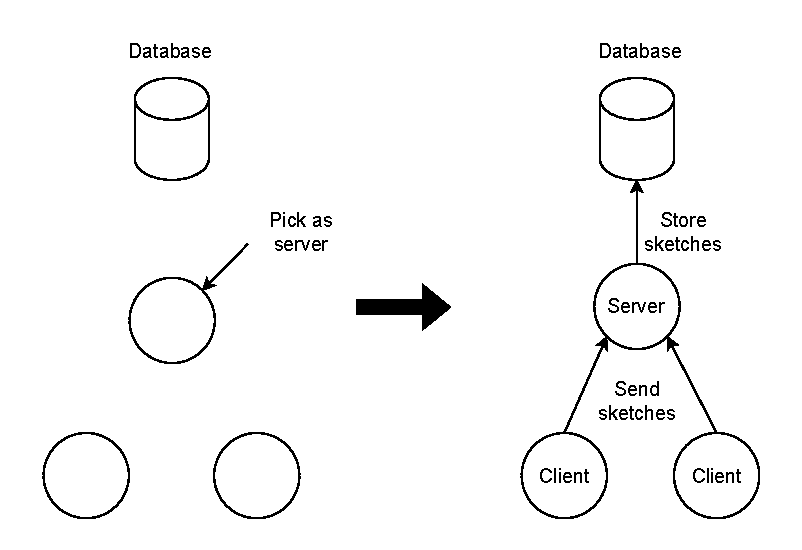
\includegraphics[scale=0.7]{architecture.pdf}
    \caption{Architecture overview}
    \label{fig:architecture}
\end{figure}

The rationale behind this set up is as follows: The goal of our system is to minimize the amount of data sent across the network, therefore the datasets should be locally processed to create a summary which is smaller in size and thus transferable over the internet. At this point, a server is not needed, since a machine can simply send the summaries to the database server to store and query the database to find similar datasets. However, as already discussed in section \ref{lsh}, pair-wise similarity calculations are costly so we use LSH for similarity search, specifically the Lazo implementation proposed by Bogatu et al. \cite{lazo}. Unfortunately, one drawback of Lazo is that the indexes are only capable of running in main memory, which we discuss in chapter \ref{chap:conclusion}. As a result, there needs to exist one central machine to store the LSH indexes. An alternative would be for all machines to store indexes, which would require all machines to retrieve new summary and update their indexes whenever new summaries enter the database, incurring unnecessary network traffic.

\section{Usage}

The system starts by letting an user from a machine boot up the server application, then letting users from client machines boot up their respective client applications, providing the application on startup with the base IP address and port where the server can be reached. Were the server application to be moved to another machine, users from client-side boot up the application again with the new IP address and port. Once the server and client are both running, user can access a graphical interface from the web browser. From there, user can choose between two primary actions: upload and query.

\begin{itemize}
    \item \textbf{Upload action}: Submit datasets for the client application to process, create summaries and send to the server via REST request to store. In the interface, user can either choose to upload a single file, by providing the path from the file system to that exact file, or user can upload an entire folder of datasets by specifying the path to that folder (figure \ref{fig:upload}). Depending on the result of the action, the UI displays a success or error message.
    \item \textbf{Query action}: Submit a dataset for the client application to process, create summaries and send to the server via REST request to query. In the interface, user provide the path to the file to be queried, the limit on how many matches to receive, the threshold at which a pair is considered a match and choose between the two query modes: join and union (figure \ref{fig:query}). If the action failed, an error will be displayed on the form interface, meanwhile a successful action will redirect the user to the result interface, where all matches are displayed in descending order of similarity score (\ref{fig:result}). 
\end{itemize}

\begin{figure}
    \centering
    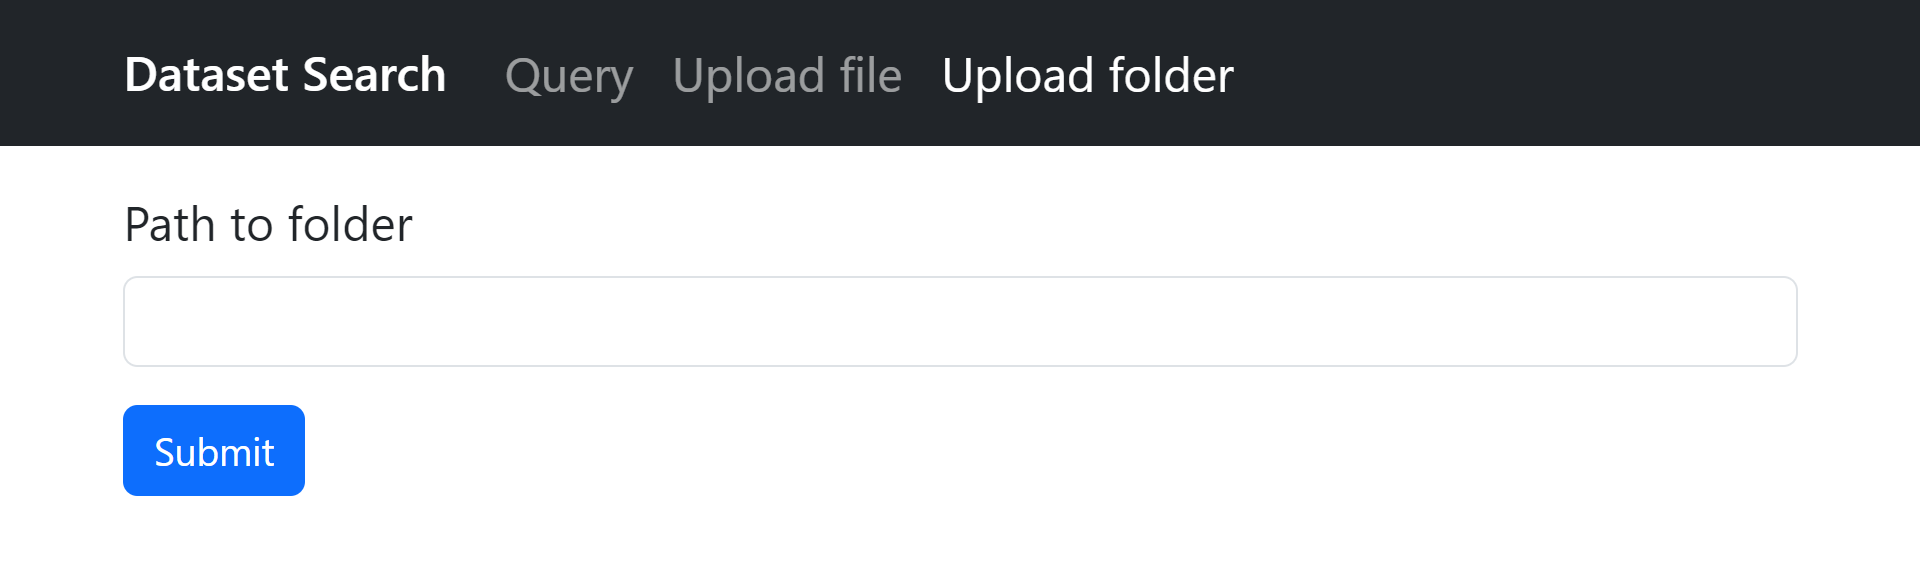
\includegraphics[width=\textwidth]{upload.png}
    \caption{Upload interface}
    \label{fig:upload}
\end{figure}

\begin{figure}
    \centering
    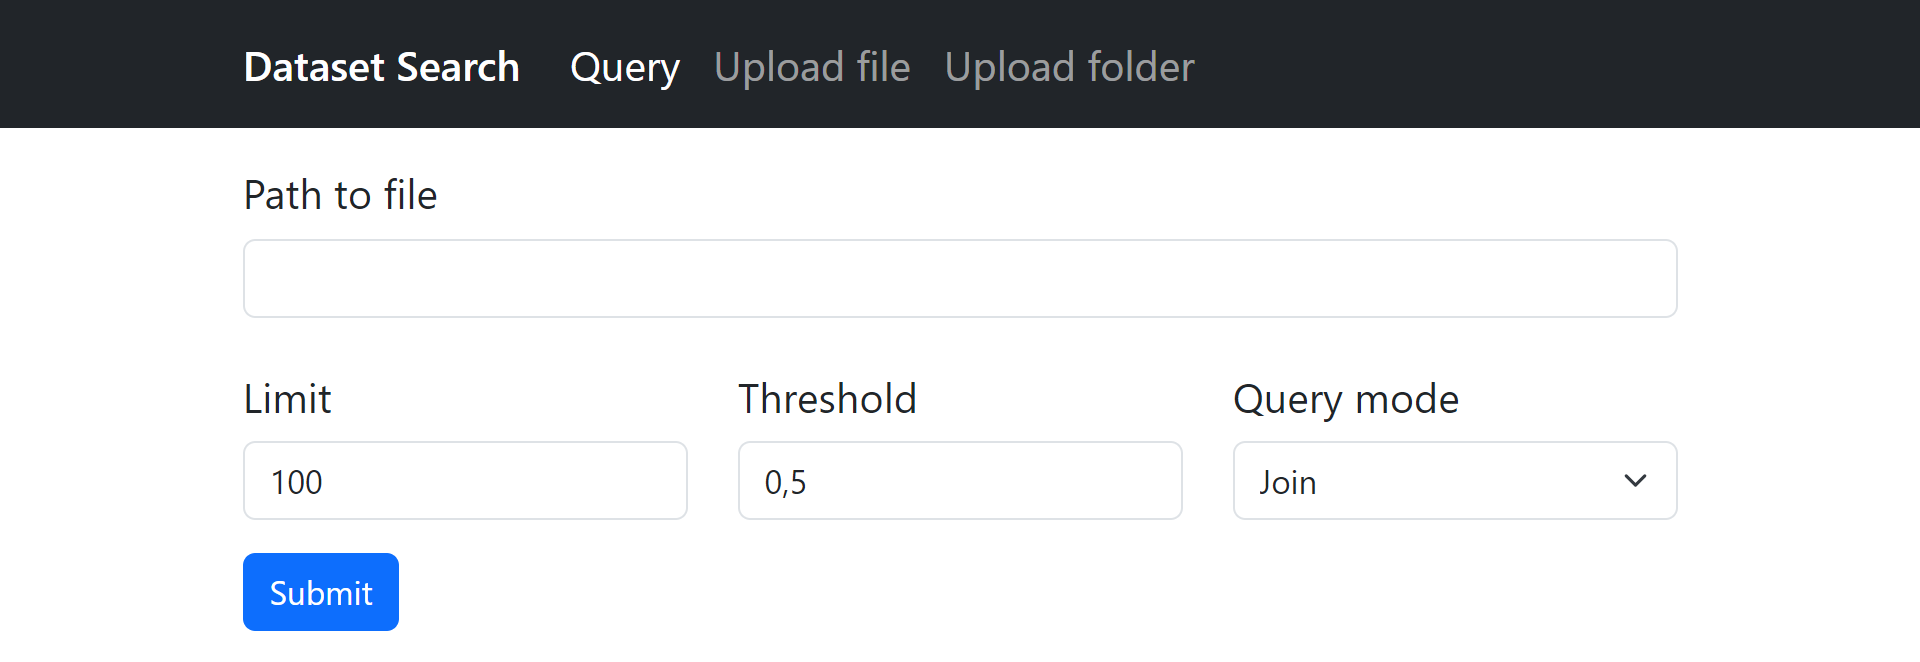
\includegraphics[width=\textwidth]{query.png}
    \caption{Query interface}
    \label{fig:query}
\end{figure}

\begin{figure}
    \centering
    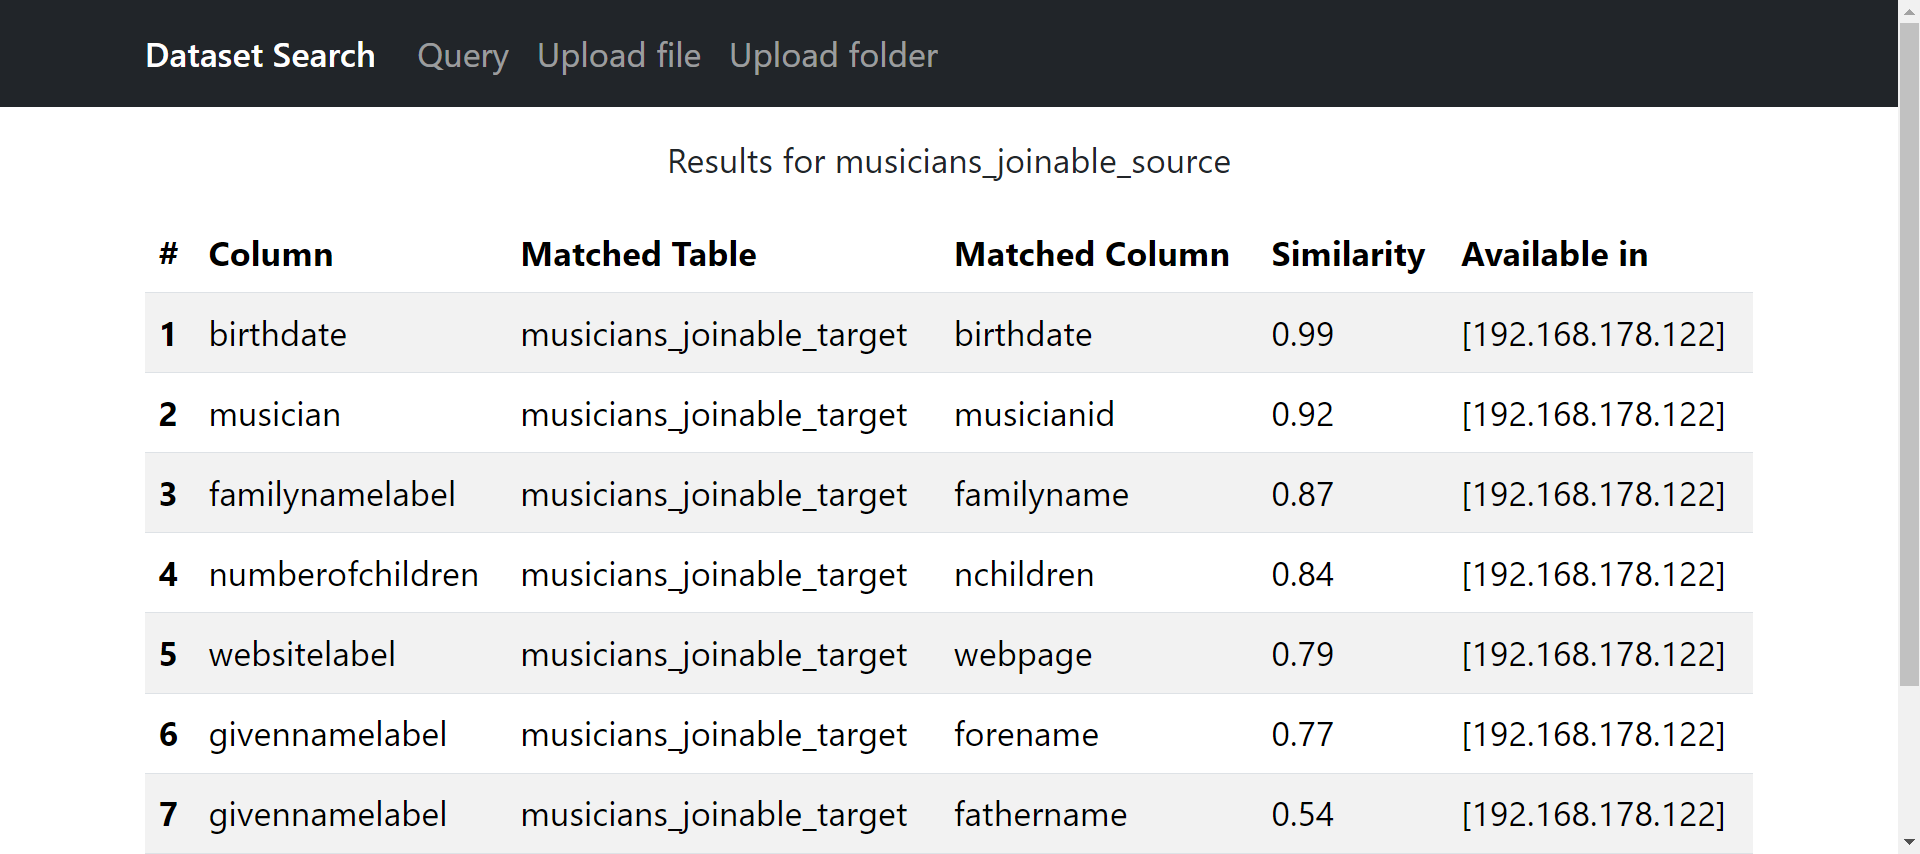
\includegraphics[width=\textwidth]{result.png}
    \caption{Result interface}
    \label{fig:result}
\end{figure}
% !TEX root =  main.tex



\chapter{Implementation}
\label{chap:implementation}
\pagestyle{plain}

In this chapter, a detailed view of the system is presented. First, the objects used to communicate between server and clients are introduced. Then, a brief introduction to MongoDB, our database of choice is given. After that, we provided the implementation of the client application and lastly the server's implementation. We make the following assumptions about the datasets we are working with: they are files in CSV format and the first row of the files contain the headers/attribute names of the datasets. The system is implemented using Java and the Spring framework.

\section{Communication Objects}

There are two main types of objects that are exchanged between client and server: dataset summaries and query results. The summaries are created from the client side and sent to the server using POST requests either to be stored or to be queried. The query results object is the response that the server returns whenever the query endpoint is accessed.

\subsection{Dataset Summaries}\label{metadata}

A dataset is summarized on a column-by-column basis. The summary of a column contain two main component: the metadata and the sketches:

\begin{itemize}
    \item \textbf{Metadata}: Provides basic information about a column of a table (listing \ref{lst:metadata}): the name of the table that this column belongs to, the name of this column, its datatype, the size/amount of elements the column contains, and a set of IP-Addresses of machines that carry this dataset. An additional id field that contains an UUID representing the table name, concatenated with the column name is associated with each metadata to uniquely identify the metadata and provide easy retrieval of all metadata of a dataset, which is discussed more in detail in the upcoming section.
    \begin{lstlisting}[caption={Preview of the metadata object}, label=lst:metadata]
class Metadata {
    // id = uuid + SEPARATOR + column_name
    // uuid is the same for all metadata of a dataset
    String id;
    String table_name;
    String column_name;
    String type;
    int size;
    int arity;
    Set<String> addresses;
}
    \end{lstlisting}
    \item \textbf{Sketches}: A set of Lazo's implementation of MinHash sketches, represented by the stored hash values and the cardinality of the set that is sketched (\ref{lst:sketches}), which the authors used to improve estimation accuracy. The sketches are generated from the sets that were mentioned in section \ref{simMeasures}.

\begin{lstlisting}[caption={Preview of the sketches object}, label=lst:sketches]
class Sketches {
    // id refers to the Metadata object
    private String id;
    private Set<Sketch> sketches;
}

class Sketch {
    SketchType type;
    long cardinality;
    long[] hash_values;
}

enum SketchType {
    TABLE_NAME, COLUMN_NAME, COLUMN_VALUE, FORMAT
}
    \end{lstlisting}
\end{itemize}

\subsection{Query Results}

This object contains a list of individual entries of result, where a result maps one metadata from the query table to one matched metadata along with the similarity score of this match (listing \ref{lst:queryResults}). The list of results are sorted in descending order of similarity scores.

\begin{lstlisting}[caption={QueryResults class and the various methods to sort, filter, and limit matches}, label=lst:queryResults]
public record QueryResults(List<SingleResult> results) {
    // Return a new QueryResults object with the results sorted by score in descending order
    public QueryResults sortResults();
    //Return a new QueryResults object with the top n highest scoring results. The results are sorted by score in descending order
    public QueryResults limitResults(int limit);
    // Return a new QueryResults object with only the results that have a score greater than or equal to the threshold
    public QueryResults withThreshold(double threshold);
}

public record SingleResult(Metadata query, Metadata candidate, double score) {}
\end{lstlisting}

\section{Database}

In order to store the metadata and sketches, MongoDB is used. This is the database of choice due to several reasons:

\begin{itemize}
    \item Replication: MongoDB is a distributed database, where the data are stored on multiple database servers. This redundancy increases data availability and provides fault tolerance in case a single database server fails.
    \item Flexible schema: MongoDB is a NoSQL database, therefore it does not store data in relational manner, but rather stored in JSON-style documents, which do not have constraint on the amount of attributes and their types. This allows us to make changes to the schema in case e.g. a new sketch type for certain types of attributes is developed without having to perform alterations to existing data to fit the new schema.
    \item Object mapping: The format MongoDB stores data in allow them to be easily converted to a Java object without the use of Object-Relational-Mappers (like OpenJPA \footnote{https://openjpa.apache.org/})
    \item Fast read: MongoDB uses index to speed up data retrieval on indexed fields, especially on id field. Since the system mostly query on id field, and the sketches are need to be read into main memory on server startup (due to Lazo's LSH index), the database provides high performance to the system.
    \item Unique index: Additionally, MongoDB also provides unique indexed, which ensure that the indexed fields do not store duplicate values. We use this feature to detect duplicate metadata. This happens when two machines contain the same dataset and both are trying to upload the summaries to the server. When duplicates are detected, they are grouped into the same metadata, with the set of addresses merged together.
\end{itemize}

In our database, there are two collections, one for the metadata and one for the for the sketches. The collections consist of documents, which are simply JSON strings in binary format mapped from the respective Java objects. An unique index is also set up on the fields table\_name, column\_name, type, size and arity of the metadata collection for reasons we mention in section \ref{profiler} and \ref{saveController}.

\section{Client Application}

In this section, we describe the two main components of the application on the client side, which are the controller and the profiler.

\subsection{Controller}

The main job of the controller (listing \ref{lst:appcontroller}) is to handle communications between user, client and server. It displays the forms to the user according to which action they want to take, retrieves the CSV files the user provide from the form, send the acquired table to the profiler to process, send the summaries to the server and displays back to the user the response that the server returned. The reading of CSV files are performed using Tablesaw \footnote{https://github.com/jtablesaw/tablesaw}, a third party library that provides column-wise reading and automatic type detection of attribute. The controller performs REST requests to the server via the WebClient class, which is a class provided by Spring Reactive Web Framework to create HTTP requests. Upon application startup, a WebClient builder takes the IP address and port of the server that the user provided from the command line argument and create an instance of the WebClient with the server's URL as base URL.

\begin{lstlisting}[caption={Preview of the controller class}, label=lst:appcontroller]
@Controller
class AppController {
    // Perform REST requests
    WebClient client;
    Profiler profiler;

    @GetMapping("/upload_file")
    public String uploadFile(...) {
        // Display form to upload a single dataset
    }

    @PostMapping("/upload_file")
    public String saveFile(Form form, ...) {
        Path path = Path.of(form.getPath());
        Table table = CSVReader.readTable(path, true);
        List<Summaries> summaries = profiler.profile(table);
        // Send summaries via POST request to /save endpoint
        client.post()
                .uri("/save")
                .bodyValue(summaries)
                .retrieve().bodyToMono(Void.class).block();
        ...
    }

    @PostMapping("/query")
    public String sendQuery(QueryForm form, ...) {
        ...
        // Send summaries via POST request to /query endpoint,
        // QueryResults are used to display the results to GUI
        QueryResults results = client.post()
                .uri(builder -> builder
                        .path("/query")
                        .queryParam("mode", form.getMode())
                        .queryParam("limit", form.getLimit())
                        .queryParam("threshold", form.getThreshold())
                        .build())
                .bodyValue(summaries)
                .retrieve().bodyToMono(QueryResults.class).block();
    }
    
}
\end{lstlisting}

\subsection{Profiler}\label{profiler}

The profiler generates the metadata of a table by iterating over its columns to get the information in section \ref{metadata}. In the current implementation, the IP-Address is the local address of the machine the application is running on, which allows distinction between machines in a local area network. While table name, column name and data type are used for similarity calculation, the column size and table's arity provide additional distinguishing information to detect duplicate datasets entering the database.

As for sketches, the profiler uses three main methods: createNameSketch(), createColumnSketch() and createFormatSketch().

\begin{itemize}
    \item createNameSketch() (listing \ref{lst:nameSketch}): used to create MinHash sketch for the table name and column name from their q-gram-sets. The q-value of 4 is used, similar to \cite{d3l}. If a string has a length smaller than 4, the input of the sketch generator would be an empty set.
    \begin{lstlisting}[caption=qGram() and createNameSketch() methods, label=lst:nameSketch]
public Set<String> qGram(String s) {
    Set<String> res = new HashSet<>();
    for (int i = 0; i < s.length() - Q + 1; i++) {
        res.add(s.substring(i, i + Q));
    }
    return res;
}

public Sketch createNameSketch(String name, SketchType type) {
    Set<String> q_gram_sets = qGram(name);
    LazoSketch lazo_name_sketch = sketch_generator.createSketch(q_gram_sets);
    return new Sketch(type, lazo_name_sketch.getCardinality(), lazo_name_sketch.getHashValues());
}
    \end{lstlisting}
    
    \item createColumnSketch() (listing \ref{lst:columnSketch}): the method creates MinHash sketches from unique values set of a column, if a column is of type String, the values are not sketched as is, but rather transformed into a set of q-grams using the qGram() method above, which help finding fuzzy matches.

    \begin{lstlisting}[caption=createColumnSketch() method, label=lst:columnSketch]
public Sketch createColumnSketch(Column column) {
    LazoSketch lazo_sketch = sketch_generator.createEmptySketch();
    if (column.type() == STRING) {
        // Iterate through the column's unique values
        for (String s: column.asSet()) {
            Set<String> shingles = qGram(s);
            sketch_generator.updateSketch(shingles, lazo_sketch);
        }
    }
    else {
        sketch_generator.updateSketch(column.asSet(), lazo_sketch);
    }
    return new Sketch(SketchType.COLUMN_VALUE, lazo_column_sketch.getCardinality(), lazo_column_sketch.getHashValues());
}
    \end{lstlisting}
    
    \item createFormatSketch(): the method creates a sketch on the set of regexs that describe all possible values of the column. The regex grammar uses the set of patterns in listing \ref{lst:patterns} as the alphabet, which is the extended patterns set from \cite{d3l} as we found their patterns are not listed in the correct order and are not discriminating enough. For each value represented as a string, algorithm \ref{alg:formatRegex} continually tokenizes the string from the beginning until the end, finding the longest starting substring to convert to a character in the alphabet. If a value matches more than one pattern, the first match from the listing is chosen. And if a character in the alphabet appears consecutively, all occurrences except the first are replaced by "+". For example, a column with the set of values \(\{Alice\;C., bob, cat, user1??\}\) would yield the regex set \(\{cwup, l, ao+\}\). 

    \begin{lstlisting}[caption=Alphabet of the regex, numbers=none, label=lst:patterns]
// Matches the start of a string with alphanumeric characters
a = ^(?:[0-9]+[a-zA-Z]|[a-zA-Z]+[0-9])[a-zA-Z0-9]*
// Matches the start of a string with capitalized characters
c = ^[A-Z][a-z]+
// Matches the start of a string with uppercase characters
u = ^[A-Z]+
// Matches the start of a string with lowercase characters
l = ^[a-z]+
// Matches the start of a string with numbers
n = ^[0-9]+
// Matches the start of a string with punctuations
p = ^\\p{Punct}+
// Matches the start of a string with whitespaces
w = ^\\s+
// Matches the start of a string with a character that is not catched by other pattern
o = .
    \end{lstlisting}

    \begin{algorithm}
    \caption{formatRegex() algorithm}
    \label{alg:formatRegex}
        \begin{algorithmic}[1]
\STATE \textbf{Input}: String $s$
\STATE \textbf{Output}: Regex string $r$ describing $s$
\STATE $r \gets ""$
\WHILE{$!s.isEmpty()$}
\STATE $char \gets$ longest substring that matches a pattern in the alphabet
\STATE $r \gets r + c$
\STATE $s \gets s.substring(char.length())$
\ENDWHILE
\STATE $r \gets $ consecutive occurrences of a character in $r$ replaced by $"+"$
\RETURN $r$
            
        \end{algorithmic}
    \end{algorithm}
    
\end{itemize}

The sketch generator is a supporting class that handles the process of reading the input set and transforming it to Lazo's implementation of MinHash sketches (LazoSketch object). As the LazoSketch only hashes input values of type string, we provide a method to convert the values to be sketched to their string representation (listing \ref{lst:sketchGenerator}). There are also two special cases where the input set is empty or is of type boolean. In case the set is empty, we return a LazoSketch containing the hash values of the empty string. If the set is a boolean set, then the string representation of the boolean values are 0 and 1.

\begin{lstlisting}[caption=The SketchGenerator class, label=lst:sketchGenerator]
public class LazoSketchGenerator {
    public LazoSketch createSketch(Iterable<?> iterable) {
        return updateSketch(iterable, createEmptySketch());
    }

    public LazoSketch createEmptySketch() {
        return new LazoSketch();
    }

    public LazoSketch updateSketch(Iterable<?> iterable, LazoSketch sketch) {
        if (!iterable.iterator().hasNext()) {
            sketch.update("");
            return sketch;
        }
        for (Object value: iterable) {
            if (value == null) sketch.update("");
            else if (value instanceof Boolean b) sketch.update(b ? "1" : "0");
            else sketch.update(value.toString().trim());
        }
        return sketch;
    }
}
\end{lstlisting}

\section{Server Application}

In this section, we describe the components of the server. First is the controller that provides the endpoint for the save action. Then we show how the sketches are stored in the LSH indexes and how the indexes are queried to retrieve similarity scores. Next, we go into details on the calculation of the WordNet similarity score. After that, we explain the way to combine all similarity scores from different measures to one single score. Finally, an optimization technique is also presented to avoid unnecessary calculations, ensuring that the server performs efficiently when there are many datasets present.

\subsection{Save Controller}\label{saveController}

In this REST controller class, a save endpoint is available to receive dataset summaries from clients. The controller communicates with the database using the MongoRepository interface from Spring framework, which provides a convenient way of database interaction by removing the need to write boilerplate code. To perform a query on a database, we need only to extend the interface with a method name that contains specific query keywords. For example:

\begin{lstlisting}[caption=Example of the the repository interface for collection of metadata, label=lst:metadataRepo]
@Repository
public interface MetadataRepo extends MongoRepository<...> {
    List<Metadata> findByIdStartsWith(String regex);
    
    @Query("{ 'table_name': ?0, 'column_name': ?1, 'type': ?2, 'size': ?3, 'arity': ?4 }")
    Optional<Metadata> findByUniqueIndex(String table_name, String column_name, String type, int size, int arity);
}
\end{lstlisting}

In listing \ref{lst:metadataRepo}, we extend MongoRepository with method findByIdStartsWith() to query for metadata whose id starts with the same string given in the input. Instead of having to provide an implementation of the method, MongoRepository automatically recognizes the keywords:

\begin{itemize}
    \item \textit{find}: Look up in the database
    \item \textit{ById}: Look for field "id" in the Metadata objects
    \item \textit{StartsWith}: Adds to the lookup condition that only id that starts with the string in the input are returned.
\end{itemize}

and construct a query out of them. In the case where a query is too complex to be built using only keywords, we can also provide the query manually in the @Query annotation, like in the findByUniqueIndex() method where we look for a single metadata that matches the unique index constraint by listing the fields' names as key and placeholders as values, which are replaced by the method's arguments when the query is executed.

When the list of Summaries objects make it to the save endpoint on the server, for each summaries (a column of a table) the controller first attempt to insert the metadata to the database before inserting the sketches to the database and to the indexes. If a DuplicateKeyException is thrown, then we know that the metadata already exists due to the unique index constraint. The existing metadata is retrieved instead and the IP address field of the metadata taken from the request is added to the existing address set in the database, indicating that the dataset is available from multiple sources (listing \ref{lst:saveController}).

\begin{lstlisting}[caption=The save controller, label=lst:saveController]
@RestController
public class SaveController {
    MetadataRepo metadata_repository;
    SketchesRepo sketches_repository;
    LSHIndex lsh_index;


    @PostMapping("/save")
    public void save(@RequestBody List<Summaries> request_objects) {
        for (Summaries request_object : request_objects) {
            try {
                metadata_repository.save(request_object.metadata());
            } catch (DuplicateKeyException e) {
                ...
                Set<String> addresses = request_object.metadata().getAddresses();
                Metadata metadata = metadata_repository.findByUniqueIndex(table_name, column_name, type, size, arity).get();
                metadata.getAddresses().addAll(addresses);
                continue;
            }
            sketches_repository.save(request_object.sketches());
            lsh_index.updateIndex(request_object.sketches());
        }
    }
}
\end{lstlisting}

\subsection{LSH index}

Once the summaries are stored in the database, they are then also immediately loaded into the LSH indexes that lie the main memory. There are currently four indexes available to correspond to the 
four sketch types available as seen in listing \ref{lst:sketches}. The insertion method (listing \ref{lst:updateIndex}) works by first recreating the LazoSketch object from the cardinality value and the hash values from the Sketch object. Then the method checks the type field from the Sketch object to see in which index should this LazoSketch be inserted to. The Lazo index also requires an object to be inserted as a key to identify the results return upon querying. Since the sketch uniquely identifies a metadata/column of the table in each index, the id of the metadata is chosen to be the key. 

\begin{lstlisting}[caption=Inserting sketches into the indexes, label=lst:updateIndex]
public clas LSHIndex {
    LazoIndex table_name_index = new LazoIndex();
    LazoIndex column_name_index = new LazoIndex();
    LazoIndex column_value_index = new LazoIndex();
    LazoIndex format_index = new LazoIndex();

    public void updateIndex(Sketches sketches) {
        for (Sketch sketch: sketches.getSketches()) {
            addSketchToIndex(sketches.getId(), sketch);
        }
    }

    public void addSketchToIndex(String id, Sketch sketch) {
        LazoSketch lazo_sketch = recreateSketch(sketch.cardinality(), sketch.hash_values());
        switch (sketch.type()) {
            case TABLE_NAME -> table_name_index.update(id, lazo_sketch);
            case COLUMN_NAME -> column_name_index.update(id, lazo_sketch);
            case COLUMN_VALUE -> column_value_index.update(id, lazo_sketch);
            case FORMAT -> format_index.update(id, lazo_sketch);
        }
    }

    public LazoSketch recreateSketch(long cardinality, long[] hash_values) {
        LazoSketch sketch = new LazoSketch();
        sketch.setCardinality(cardinality);
        sketch.setHashValues(hash_values);
        return sketch;
    }
}
\end{lstlisting}

Since the indexes are stored in memory, upon starting the application, all sketches also have to be loaded from the database (listing \ref{lst:loadIndex}). While this is inefficient, we argue using evaluation statistics that the footprint of the sketches are small enough to be read all at once and the server startup is not a common operation, therefore the loading process does not compromise the usability of the system.

\begin{lstlisting}[caption=Load all sketches into indexes during initialization, label=lst:loadIndex]

SketchesRepo sketches_repository;

public LSHIndex() {
    loadIndexes();
}

private void loadIndexes() {
    for (Sketches sketches: sketches_repository.findAll()){ 
        updateIndex(sketches);
    }
}
\end{lstlisting}

Now, in order to query the indexes, the LazoIndex class provides a method query() that takes the query LazoSketch as input, as well as the threshold of similarity above which another LazoSketch is considered a candidate. The method then returns a set of LazoCandidate, which is just a wrapper object for the key that correspond to the LazoSketch that was inserted and three scores: Jaccard coefficient, set containment of the query in candidate and the set containment in the opposite direction (listing \ref{lst:queryIndex}).

\begin{lstlisting}[caption=The query() method that LazoIndex provided, label=lst:queryIndex]
public class LazoIndex {
    Set<LazoCandidate> query(LazoSketch sketch, float threshold)
}

public class LazoCandidate {
    public final Object key;
    // Jaccard coefficient
    public final float js;
    // Set containment of query in candidate
    public final float jcx;
    // Set containment of candidate in query
    public final float jcy;

    public LazoCandidate(Object key, float js, float jcx, float jcy) {
        this.key = key;
        this.js = js;
        this.jcx = jcx;
        this.jcy = jcy;
    }
}
\end{lstlisting}

When we call the query() method, for each candidate returned, we check the key (id of corresponding metadata) of the candidate to make sure the candidate is not the from the same table as the query input. This is achievable thanks to the UUID present in the id that identifies unique a table. Therefore, in order to check whether two metadata/columns come from the same table or not, we only need to check the UUID prefix of the metadata. Then, we retrieve the candidate metadata from the key of the LazoCandidate object and wrap the three scores (js, jcx and jcy) into a separate object. All the metadata are finally mapped to their corresponding scores for further query processing. The algorithm is shown in \ref{alg:queryIndex}.

\begin{algorithm}
    \caption{Querying the LSH index}
    \label{alg:queryIndex}
    \begin{algorithmic}[1]
\STATE \textbf{Input}: Index to be queried $I$, LazoSketch $s$, sketch identifier $id$, threshold $t$
\STATE \textbf{Output}: Map $C$ of metadata candidates to its score
\STATE $C \gets Map()$
\FOR{$candidate$ in $index.query(s, t)$}
\STATE $candidate\_id = candidate.key$
\IF{$candidate\_id$ belongs to same table as $id$}
\STATE continue
\ENDIF
\STATE $candidate\_metadata \gets findById(candidate\_id)$
\STATE $score \gets new Score(candidate.js, candidate.jcx, candidate.jcy)$
\STATE $C.put(candidate\_metadata, score)$
\ENDFOR
\RETURN $C$
    \end{algorithmic}
\end{algorithm}

\subsection{Wordnet Similarity Calculator}

As mentioned before in section \ref{simMeasures}, while syntactic similarity can be calculated from the LSH indexes, semantic similarity calculation is achieved using WordNet database, and more specifically with the Wu-Palmer algorithm. For this, we use a third party library \footnote{https://github.com/dmeoli/WS4J} that provides an implementation of the Wu-Palmer algorithm as a base to compute our metric.

One problem with using WordNet is, however, the database only contains words in its base form: i.e. singular nouns, verbs that are not conjugated. As a result, performing the Wu-Palmer algorithm on any words that are not in their base form will yield a similar score of 0. Therefore, a way is needed to first transform a word back to its base form before calculation. For this task, we employ Stanford's natural language processing (NLP) library \footnote{https://stanfordnlp.github.io/CoreNLP/}, which contains lemmatization algorithm. This is different from word stemming algorithms like Porter stemmer \footnote{https://snowballstem.org/algorithms/porter/stemmer.html} since stemming may not actually return a real English word, which is necessary requirement for our application.

We then proceed to extend the semantic similarity between words to the entire table and attribute name, which can be multiple words long. Firstly, the string representation of the name is tokenized into a list of individual string by splitting it around whitespaces or underscores, which are common word separator in names (listing \ref{lst:tokenize}).

\begin{lstlisting}[caption=tokenize() method, label=lst:tokenize]
public List<String> tokenize(String s) {
    \\ regex denotes consecutive occurences of whitespaces or underscores
    return Arrays.asList(s.split("\\s+|_+"));
}
\end{lstlisting}

Then, the tokenized words are wrapped in a sentence class from NLP's library so that the words can be lemmatized. After that, the stop words (stored in a predefined list) are removed from the word list as they do not contribute to the semantic relatedness of the name. We do not remove the stop words before lemmatization since NLP library uses context of other words to determine the part of speech for correct word transformation. Finally, the algorithm from section \ref{wordnet} is applied. The entire process is describe in algorithm \ref{alg:wordnet}:

\begin{algorithm}
    \caption{WordNet similarity of table/attribute names}
    \label{alg:wordnet}
    \begin{algorithmic}[1]
\STATE \textbf{Input}: Strings $name1$ and $name2$
\STATE \textbf{Output}: Similarity score $name\_sim$
\STATE $sentence1 \gets tokenize(name1)$
\STATE $sentence2 \gets tokenize(name2)$
\STATE $lemma1 \gets sentence1.lemmas()$
\STATE $lemma2 \gets sentence2.lemmas()$
\STATE $removeStopWords(lemma1)$
\STATE $removeStopWords(lemma2)$
\STATE $name\_sim=0$
\FOR{$word1$ in $lemma1$}
\STATE $word\_sim\_max=0$
\FOR{$word2$ in $lemma2$}
\STATE $word\_sim=wuPalmer(word1, word2)$
\IF{$word\_sim == 0$}
\STATE $word\_sim = levenshteinSimilarity(word1, word2)$
\STATE $word\_sim\_max=max(word\_sim\_max, word\_sim)$
\ENDIF
\ENDFOR
\STATE $name\_sim+=word\_sim\_max$
\ENDFOR
\FOR{$word2$ in $lemma2$}
\STATE $word\_sim\_max=0$
\FOR{$word1$ in $lemma1$}
\STATE Repeat steps 13 - 17
\ENDFOR
\STATE $name\_sim+=word\_sim\_max$
\ENDFOR
\STATE $name\_sim = name\_sim \; / \; (lemma1.size() + lemma2.size())$
\RETURN $name\_sim$
    \end{algorithmic}
\end{algorithm}

\subsection{Measure Object}

In order to differentiate the similarity scores of different similarity measurements, we wrap the score into a Measure object that contains the score, the type of measure this score represents, and the weighting of this score (listing \ref{lst:measure}), which is taken into consideration when the scores are aggregated together. 

\begin{lstlisting}[caption=The measure object,label=lst:measure]
public record Measure(MeasureType measures, double score, int weight) {}

public enum MeasureType {
    COLUMN_VALUE, COLUMN_FORMAT, COLUMN_NAME_QGRAM, TABLE_NAME_QGRAM, COLUMN_NAME_WORDNET, TABLE_NAME_WORDNET
}
\end{lstlisting}

The score's weight of a measure depends on what type of measure it is and whether the query mode is join or union. The intuition behind the weighting system is that some types of similarity measures may play a more significant role in telling the degree of relatedness than others. For example, in the TPC-H \footnote{https://www.tpc.org/tpch/} schema, the table Orders and Customer are joinable with each other through the attribute custkey. However, it is apparent that the two words orders and customers are not that related to each other. Therefore, it is sensible to not weight the similarity of the table names as high as other measures during aggregation, but rather focus more weight on the column values overlap to detect the foreign key constraint. On the other hand, imagine the Orders table belong to a company, where every year the company creates a new Orders table to keep track of orders for only that year. Then they may name each Orders table Orders\_2020, Orders\_2021, ... etc. Now, we want find all the Orders table to union them to one single table, then the table name would be of much more importance than column values overlap, since the order records of each year does not necessarily have any overlap between each other. For this reason, the weighting of the measures also differ in case of join or union.

For each pair of query - candidate column, to get all of the measures calculated between them, we wrap them again in the Measures object (listing \ref{lst:measures}):

\begin{lstlisting}[caption=The Measures object, label=lst:measures]
public class Measures {
    List<Measure> measures;

    public void addMeasure(Measure measure) {
        if (measures.stream().anyMatch(m -> measure.measure() == m.measure())) {
            throw new RuntimeException("Measure already exist in the list");
        }
        measures.add(measure);
    }

    public double weightedAverage() {
        double result = 0;
        double total_weight = 0;
        for (Measure measure: measures) {
            double weight = measure.weight();
            result += measure.score() * weight;
            total_weight += weight;
        }
        return result / total_weight;
    }
}
\end{lstlisting}

Given the list of measures, this class aggregates the scores using weighted sum:

\[score(query, candidate) = \frac{\sum_{m \in measures} w_m \cdot sim_m(query, candidate)}{\sum_{m \in measures} w_m}\]

Since all calculated scores are in the range 0 to 1, the aggregated score also ranges from 0 to 1.

\subsection{Query Controller}

In main endpoint provided in this REST controller class is the query endpoint, where it receives the summaries of the query dataset along with three additional query parameters: query mode (union or join), limit (number of matches returned) and threshold at which an aggregated score is considered a match. The algorithm (\ref{alg:queryTable}) works as follows: in order for the query dataset to be discoverable by the LSH index, we first attempt to insert the summaries into the appropriate collections inside the database as well as inserting the sketches to the indexes (line 4-11). Here, it can happen that the dataset that the user is trying to query already existed in the database, so a DuplicateKeyException will be thrown. The insert attempt is stopped and the summaries from the database are used instead. To retrieve the summaries from the database, the unique index is used (line 15-18)). Notice we cannot lookup a dataset using the query table's UUID, as they are generated differently from the one in the database. After having the database and LSH indexes set up for the query, we call the queryColumn() method to find candidates for the individual columns of the table, as all of our similarity measures work on column level. The list of all candidates from all columns are then stored in a QueryResults object and depending on the query parameters, candidates with scores below threshold are removed and/or only top-k candidates are retained. The second to last step is to removed the query's summaries that might have been added to the database and LSH indexes from the beginning. Finally, the QueryResults object is then sent back to the client with the scores sorted from highest to lowest.

\begin{algorithm}
    \caption{queryTable() algorithm}
    \label{alg:queryTable}
    \begin{algorithmic} [1]
\STATE \textbf{Input}: Summaries list $S$, query mode $m$, limit $l$, threshold $t$ 
\STATE \textbf{Output}: Query result $R$
\STATE $existed \gets false$
\FOR{$summaries$ in $S$}
\STATE \textbf{try} insert $summaries.metadata$ and $summaries.sketches$ to database
\STATE \textbf{catch} DuplicateKeyException \textbf{do}
\STATE \; \; $existed \gets true$
\STATE \; \; \textbf{break}
\STATE \textbf{end catch}
\STATE insert $summaries.sketches$ to LSH indexes
\ENDFOR
\IF{$!existed$}
\STATE $columns \gets$ all metadata from $S$
\ELSE
\STATE $columns \gets Array()$
\FOR{$metadata\_request$ in all metadata from $S$}
\STATE $metadata\_db \gets findByUniqueIndex(indexed \; fields \; of \; metadata\_request)$
\STATE $columns.add(metadata\_db)$
\ENDFOR
\ENDIF
\STATE $R \gets QueryResult()$
\FOR{$column$ in $columns$}
\STATE $R.addAll(queryColumn(column, m))$
\ENDFOR
\IF{$!existed$}
\STATE remove query's summaries from database and LSH indexes
\ENDIF
\STATE sort $R$
\RETURN $R.withThreshold(t)$
    \end{algorithmic}
\end{algorithm}

On the column level, we differentiate between two main categories of similarity measures to perform the calculations: WordNet similarity (on table names and column names) and LSH-based similarity (on table names, column names, value sets overlap and format overlap) (listing \ref{lst:queryColumn}). In any combinations of measures used, the data types is always the first filter to be used as per section \ref{schemaSim}. Since the data types of the attribute is derived automatically from CSV file by Tablesaw, and without an official schema provided, the attribute type is ambiguous anyway. Therefore, we define classes of data types defined by Tablesaw that are similar to each other, so that two columns with different types but belong in the same class are still considered a match:

\begin{itemize}
    \item \textbf{"Stringy" types}: Text, String
    \item \textbf{Whole types}: Integer, Boolean, Long, Short
    \item \textbf{Decimal types}: Double, Float
    \item \textbf{Temporal types}: Local date, Local date time, Local time
\end{itemize}

All of the given data types correspond to a class in Java, with the Text data type also represented as Java's string type. We define boolean to belong into the whole types with the intuition that in certain datasets, booleans are not represented in its own type, but rather described by 0s and 1s. Therefore, we group them together into the same types as number, and also sketch as number as seen in section \ref{profiler}. While this can cause false positive matches, we hope that by incorporating multiple measures together to obtain a score, the amount of false positives are reduced.

\begin{lstlisting}[caption=Overview of the queryColumn() method, label=lst:queryColumn]
// metadata: query column
// is_join: true if query mode is join, else union mode
// query_measures: list of similarity measures
public QueryResults queryColumn(Metadata metadata, boolean is_join, List<MeasureType> query_measures) {
    QueryResults results = new QueryResults(new ArrayList<>());
    if (MeasureType.onlyWordNet(query_measures))
        results.addAll(onlyWordNetQuery(metadata, query_measures, is_join));
    else if (MeasureType.onlyLSH(query_measures))
        results.addAll(onlyLSHQuery(metadata, query_measures, is_join));
    else
        results.addAll(mixedQuery(metadata, query_measures, is_join));
    return results;
}
\end{lstlisting}

Now, if we wish to only find similar columns based on the WordNet similarity measures (algorithm \ref{alg:onlyWordnet}), the first step is to retrieve all the metadata from the database that do not belong to the same table as the query column and share a similar types with the query column's data type. Then, for each candidate, we apply algorithm \ref{alg:wordnet}, once per WordNet measures present, to calculate the score, wrap the score in the Measure object with the weight assigned for that specific measure and query mode, and add them to the list of measures. Finally, the aggregated score is calculated from all the measures, wrapped in the SingleResult object, and added to the query results.

\begin{algorithm}
    \caption{Query columns based only on WordNet measures}
    \label{alg:onlyWordnet}
    \begin{algorithmic}[1]
\STATE \textbf{Input}: Metadata of query column $q$, list of similarity measures $query\_measures$, query mode $m$
\STATE \textbf{Output}: Query results $R$
\STATE $table\_id \gets$ first part of $q.id$ 
\STATE $candidates \gets findByIdNotStartsWithAndSimilarType(table\_id, q.type)$
\FOR{$candidate$ in $candidates$}
\STATE $measures\_list \gets Measures()$
\FOR{$measure\_type$ in $query\_measures$}
\STATE $score \gets calculateScore(q, candidate)$
\STATE $weight \gets$ weight according to $measure\_type$ and $m$
\STATE $measure \gets Measure(measure\_type, score, weight)$
\STATE $measures\_list.add(measure)$
\ENDFOR
\STATE $R.add(q, candidate, measures\_list.aggregate())$
\ENDFOR
    \end{algorithmic}
\end{algorithm}

On the other hand, if a column is only queried based on only certain LSH indexes, the algorithm differs slightly (algorithm \ref{alg:onlyLSH}). First, from each index that needs to be queried, the candidates are retrieved, unioned, and filtered for only similar data types. To keep track of which candidates are from which index, we map the measure type to its respective candidates. Then, for each candidate from the union set, the score from the all indexes that take part in the query are returned. If a column is a candidate in one index A but not in the other index B, then we set the score of that column coming from index B to be 0. After that, the algorithm works the same as algorithm \ref{alg:onlyWordnet}.

\begin{algorithm}
    \caption{Query columns based only on LSH indexes}
    \label{alg:onlyLSH}
    \begin{algorithmic}[1]
\STATE \textbf{Input}: Metadata of query column $q$, list of similarity measures used $query\_measures$, query mode $m$
\STATE \textbf{Output}: Query results $R$
\STATE $candidates\_map \gets$ mapping from $query\_measures$ to the respective candidates
\STATE $candidates \gets$ union of all candidates from $candidates\_map$, filtered by data type
\FOR{$candidate$ in $candidates$}
\STATE $measures\_list \gets Measures()$
\FOR{$measure\_type$ in $query\_measures$}
\STATE $score \gets candidates\_map.get(measure\_type).scoreOf(candidate)$
\STATE $weight \gets$ weight according to $measure\_type$ and $m$
\STATE $measure \gets Measure(measure\_type, score, weight)$
\STATE $measures\_list.add(measure)$
\ENDFOR
\STATE $R.add(q, candidate, measures\_list.aggregate())$
\ENDFOR
    \end{algorithmic}
\end{algorithm}

In the case where both categories of similarity of measures are used, then we first follow algorithm \ref{alg:onlyLSH} to retrieve the candidates from the LSH indexes first, since they would filter out much more columns than relying solely on the data types like in algorithm \ref{alg:onlyWordnet}. Then, the WordNet calculations are performed only on the indexes' candidates and added to the list of measures as usual.

While the attempt of filtering out data types in algorithm \ref{alg:onlyWordnet}, or querying the LSH indexes first in algorithm \ref{alg:onlyLSH} reduces the amount of potential candidates before having to apply the WordNet calculation, this step still requires a costly pairwise computation between the query column and all candidates, which can cause a performance bottleneck if the amount of candidates are high. Therefore, it is favorable to avoid this step when it is possible. Notice that when a query request is sent to the server, there is also a query parameter for a threshold, where a candidate becomes a match. If the user set this threshold at 1.0 for example, and a candidate column has one type of measure whose score is lower than 1.0, then it becomes redundant to consider the score of other types of measures, as this column will not become a match anyway.

To formalize this, we define $M$ to be the set of measures used for querying, $M_x$ the set of measures whose scores have been calculated and $M_y = M \setminus M_x$ the set of measures that have not been calculated, $w_m$ the weight of measure $m$, $sim_m$ the similarity score of measure $m$ between the query column and a candidate, $t$ the threshold. A candidate is not a match when the aggregated score is below threshold $t$:

\begin{align*}
   & \frac{\sum_{m \in M} w_m \cdot sim_m}{\sum_{m \in M} w_m} < t \\
   \iff & \sum_{m \in M} w_m \cdot sim_m < t \cdot \sum_{m \in M} w_m \\
   \iff & \sum_{m \in M_x} w_m \cdot sim_m + \sum_{m \in M_y} w_m \cdot sim_m < t \cdot \sum_{m \in M} w_m \\
   \iff & \sum_{m \in M_y} w_m \cdot sim_m < t \cdot \sum_{m \in M} w_m - \sum_{m \in M_x} w_m \cdot sim_m
\end{align*}

The maximum value of any similarity score is 1, so we set $sim_m$ to 1 to find out the stop point for the algorithm:

\[\sum_{m \in M_y} w_m < t \cdot \sum_{m \in M} w_m - \sum_{m \in M_x} w_m \cdot sim_m\]

All the variables in the equation are known at the time of score calculation. We suggest the following optimization algorithm (\ref{alg:optimization}) to add to algorithms \ref{alg:onlyWordnet} and \ref{alg:onlyLSH} as well as the mixed version of them, for example after line 7. When we notice the current candidate is already below the threshold, we immediately break out of the loop and not add the candidate to the QueryResults object. 

\begin{algorithm}
    \caption{Optimization algorithm}
    \label{alg:optimization}
    \begin{algorithmic}[1]
\STATE \textbf{Input}: List of processed similarity measures $query\_measures\_x$, list of unprocessed similarity measures $query\_measures\_x$, list of calculated scores $measures$, threshold $t$
\STATE \textbf{Output}: Boolean $b$ indicating if the algorithm should stop
\STATE $total\_weight \gets query\_measures\_x.sumWeights() + query\_measures\_y.sumWeights()$
\STATE $remaining\_weight = query\_measures\_y.sumWeights()$
\STATE $current\_score = measures.aggregate()$
\RETURN $remaining\_weight < t \cdot total\_weight - current\_score$
    \end{algorithmic}
\end{algorithm}
% !TEX root =  main.tex



\chapter{Experimental Evaluation}
\label{chap:experimentalevaluation}
\pagestyle{plain}

In this chapter, we conduct a performance evaluation of the implementation, focusing on the following questions:

\begin{itemize}
    \item How compact are the size of the datasets' summaries?
    \item How long does it take to generate the summaries?
    \item How accurate are the query results?
    \item What is the impact of the in-memory LSH-Indexes on startup time?
    \item What is the impact of the optimization algorithm?
\end{itemize}

All tests are performed on a machine running Windows 11 with 16 GB of RAM, and 11th Gen Intel Core i7-1165G7 @ 2.80GHz processor. The LSH indexes are configured with threshold of 0.7 and MinHash size of 128.

\section{Datasets}

The three datasets used are TPC-DI, WikiData, and synthesized Open Data. The first two datasets were provided by Valentine \cite{valentine}, while the third one by \cite{tusZhu}.

TPC-DI ($\sim$35MB) is a synthetic dataset used for data integration benchmark. In \cite{valentine}, the authors created schema matching situations by taking the \textit{Prospect} table from TPC-DI 1.1.0 with a scale factor of three, and split the table in various ways: depending on if the situations were join or union, the table is horizontally or vertically split, with varying degree of overlaps between split instances. In some variants, noises were also added to the instances and schemas, i.e, typos, additional characters added or removed from the table name or a value to differentiate the split versions from each other. For our experiments, we random select 3 split table pairs for each schema matching case presented in the paper: joinable, semantically-joinable, unionable and view-unionable. Each table varies from 11 to 22 columns and 7492 to 14983 rows.

WikiData ($\sim$10MB) is a real world dataset that is used for Wikimedia projects. The authors focused on the table \textit{musicians} in the dataset and manually created split pairs of the table for each matching scenarios. In order to replicate a real-life situation, column names are replaced with synonyms (e.g. partner $\rightarrow$ spouse), and values were change to alternative versions (e.g. Elvis Presley $\rightarrow$ Elvis Aaron Presley). Each table varies from 13 to 20 columns and 5423 to 10846 rows.

The synthesized Open Data dataset from \cite{tusZhu} ($\sim$1,1GB) is used exclusively for union scenario. The tables were generated from a base of 32 tables from Canadian and UK open government data using random projections and selections. Each table ranges from 1 to 40 columns and about 100 to 10000 rows.

\section{Metrics}

Due to varying methodologies in research papers, we employ three metrics to measure the effectiveness of our implementation. The first metric of choice is $Recall@ground\_truth$ from \cite{valentine}:

\[Recall@ground\_truth = \frac{\text{\# of top-k matches}}{\text{k}}\]

where k is the size of the ground truth. This metric is chosen since it shows the ranking's quality of the top relevant results with respect to the ground truth. We use this metric mainly on the first two datasets.

This metric is however not employed in \cite{d3l}, whose implementation we would like to compare with, as it is most similar to ours. There, the system returns ranked matches between tables and not columns. Consequently, the metrics they used: $Precision@k$ and $Recall@k$ are not fully compatible with ours. Nevertheless, we still measure $Precision@k$ and $Recall@k$ on the third dataset (which \cite{d3l} also used) to show that the trends in our diagram as k grows match those in their implementation.

\section{Single Similarity Measure}

First, we compare how each similarity measure fares when being executed in isolation. The result of the experiment performed on the TPC-DI and WikiData datasets is shown in figure \ref{fig:singleMeasure} as a candlestick diagram, depicting the minimum, 1st quartile, 3rd quartile and maximum value of the results. The average results are shown in table \ref{tab:averageRecallSingleMeasure}. Both table name measures that rely on syntactic and semantic similarity perform noticeably worse than other measures, recalling only 7\% to 14\% of matches on average for each matching scenario. This is understandable, as using table name alone to find matches would return all attributes in that table, ignoring the similarities on the column-level. Conversely, the column name measure that uses WordNet for semantic similarity show the highest result, indicating a high correlation between the attribute name and its joinablity/unionability

\begin{table}[ht]
    \centering
    \begin{tabular}{|c|c|}
        \hline
        Measures  & Average \\
        \hline
        Table name WordNet & 0.14 \\
        Column name WordNet & 0.65 \\
        Table name q-gram & 0.07 \\
        Column name q-gram & 0.31 \\
        Values set overlap & 0.48 \\
        Value format overlap & 0.3 \\
        \hline
    \end{tabular}
    \caption{Average $recall@ground\_truth$ of individual measures}
    \label{tab:averageRecallSingleMeasure}
\end{table}

\begin{figure}[ht]
    \centering
    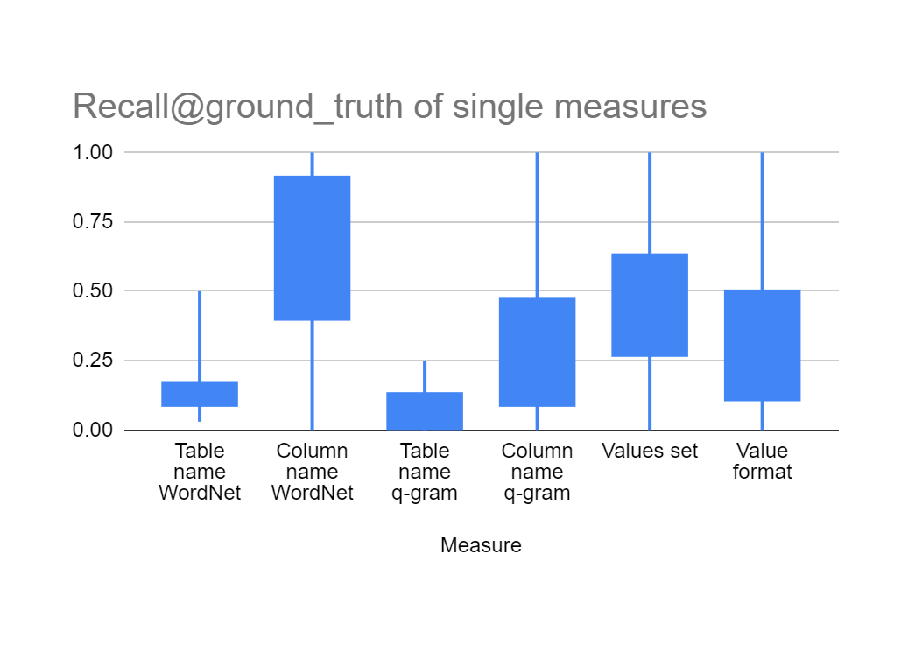
\includegraphics[scale=0.6]{singleMeasure.pdf}
    \caption{Effectiveness of similarity measures when used in isolation}
    \label{fig:singleMeasure}
\end{figure}

\section{Combined Similarity Measure}\label{combinedMeasures}

To evaluate the effectiveness of the similarity measures when aggregated, we measured $Recall@ground\_truth$ on the TPC-DI and WikiData datasets, allowing for comparison with the schema matching techniques in \cite{valentine}. $Precision@k$ and $Recall@k$ were measured on the synthesized Open Data dataset with k ranging from 1 to 400, allowing for comparison with \cite{d3l}. Precision and Recall at each k are the averages computed by perform 20 randomly selected query tables from the dataset. The similarity measures are combined in two different ways: LSH only and mixed:

\begin{itemize}
    \item LSH only: Use only scores from the LSH indexes (table name q-gram, column name q-gram, values set, values format) to aggregate the results.
    \item Mixed: Instead of using table name q-gram and column name q-gram, we use WordNet for table name and column name calculation, while keeping the values set and values format from the LSH indexes like above.
\end{itemize}

Separating the combined measures this way allow us to see whether the additional process of pair-wise semantic WordNet calculation improve the outcomes or not. Additionally, we also want to test if our hypothesized weighted scheme yield better results. Therefore, for each of the two combined measures proposed above, we split the experiment into two weighting schemes: average and weighted average. Average weight means all similarity measures have the same weight when aggregated, while the measures in the weighted average scheme are provided the following weights (table \ref{tab:weights}), which were set up following the intuition from section \ref{measureObject}.

\begin{table}[ht]
    \centering
    \begin{tabular}{|c|c|c|}
         \hline
         & Join mode & Union mode \\
         \hline
         Table name & 0.1 & 0.1\\
         Column name & 0.25 & 0.3 \\
         Values set & 0.4 & 0.2 \\
         Value format & 0.25 & 0.4 \\
         \hline
    \end{tabular}
    \caption{Weighting schema}
    \label{tab:weights}
\end{table}

The results of the experiment on TPC-DI and WikiData can be derived from figure \ref{fig:recallAtGT} and table \ref{tab:averageRecallCommbineMeasure}. We can see that the mixed variants perform on average 11\% to 17\% better than the LSH-only variants, confirming that the semantics indicate higher relatedness than purely syntax. Interestingly, the experiment also showed that the weightings have marginal difference on the outcomes in comparison to the average weighting scheme, performing only slightly better in the LSH-only combinations, and worse in the mixed combinations. This may be explained by the small variance between each weights, making the difference in the contributions of each similarity measure not too pronounced. Therefore, more experiments on different weights should be conducted. Nevertheless, the efficacy of our system falls in line with other schema matching techniques introduced in \cite{valentine}, while running on average much faster (hundreds of milliseconds to a few seconds, in comparison to hundreds of seconds).

\begin{table}[ht]
    \centering
    \begin{tabular}{|c|c|}
        \hline
        Measures  & Average \\
        \hline
        LSH average & 0.51 \\
        LSH weighted & 0.52 \\
        Mixed average & 0.68 \\
        Mixed weighted & 0.63 \\
        \hline
    \end{tabular}
    \caption{Average $recall@ground\_truth$ of combined measures}
    \label{tab:averageRecallCommbineMeasure}
\end{table}

\begin{figure}[ht]
    \centering
    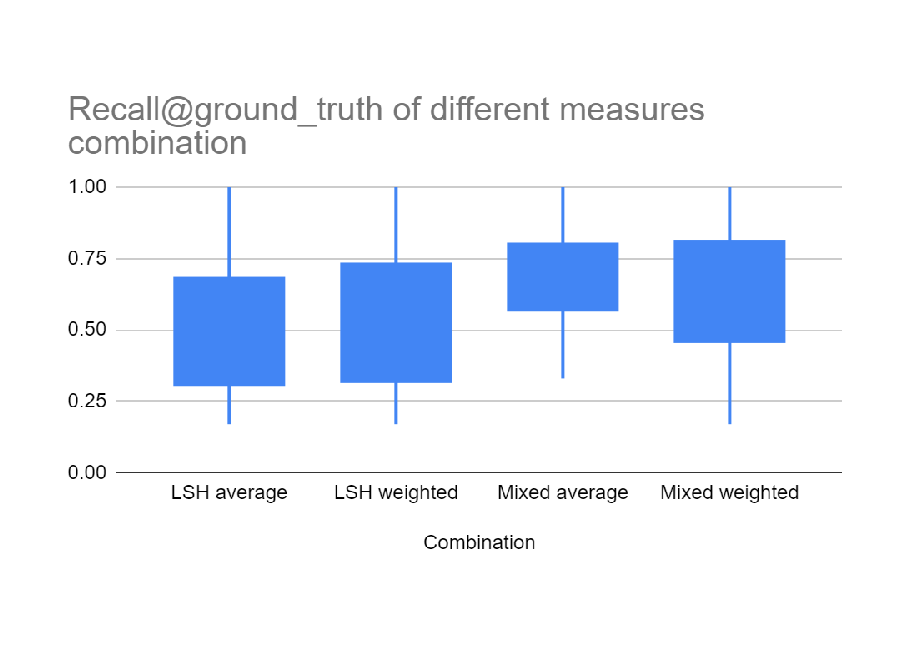
\includegraphics[scale=0.6]{recallAtGT.pdf}
    \caption{Effectiveness of similarity measures when combined}
    \label{fig:recallAtGT}
\end{figure}

As for synthesized Open Data, we show the $Precision@k$ and $Recall@k$ for varying k in figure \ref{fig:precisionAtK} and \ref{fig:recallAtK}, where precision declines linearly from around 0.85 to 0.4 and recall grows from 0.01 to 0.7 as k goes from 1 to 400. Here, the differences between each variant of the combined measures are even less pronounced, ranging from 1\% to 3\%. This also showed that the weights we used for the experiments were not effective in improving accuracy. Still, at k = 50, the system managed to return results with over 0.75 precision, suggesting that the results at the top are mostly relevant matches. Comparing our result with that of \cite{d3l}, their implementation displayed similar trends, but maintained a higher precision at higher k values than ours. This could be due to several factors: 1) they implements dynamic weighting system such that when calculating the score between a query and a candidate, it also considers the score of other candidates to determine if a similarity measure carries strong relatedness signal; 2) The MinHash size used for their LSH indexes were twice as large as ours (256), providing better performance at the cost of additional storage space; 3) Moreover, we also used a variant of Lazo's MinHash sketch that uses a technique called Optimal One-Hash-Permutation \cite{ooph} to reduce sketching time, but also comes with the downside of lower effectiveness.

\begin{figure}[ht]
    \centering
    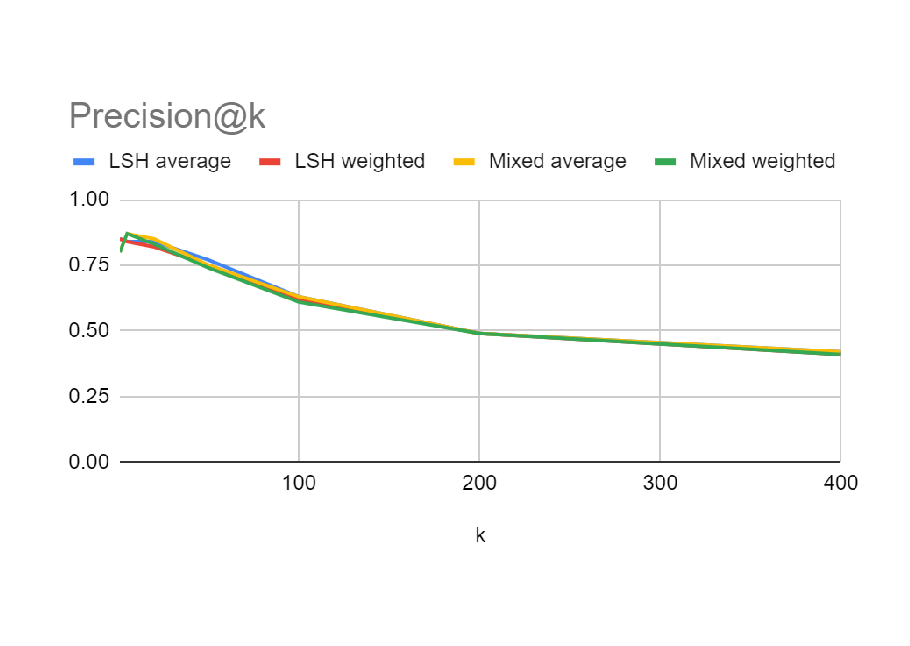
\includegraphics[scale=0.6]{PrecisionAtK.pdf}
    \caption{Precision at various top-k ranking}
    \label{fig:precisionAtK}
\end{figure}

\begin{figure}[ht]
    \centering
    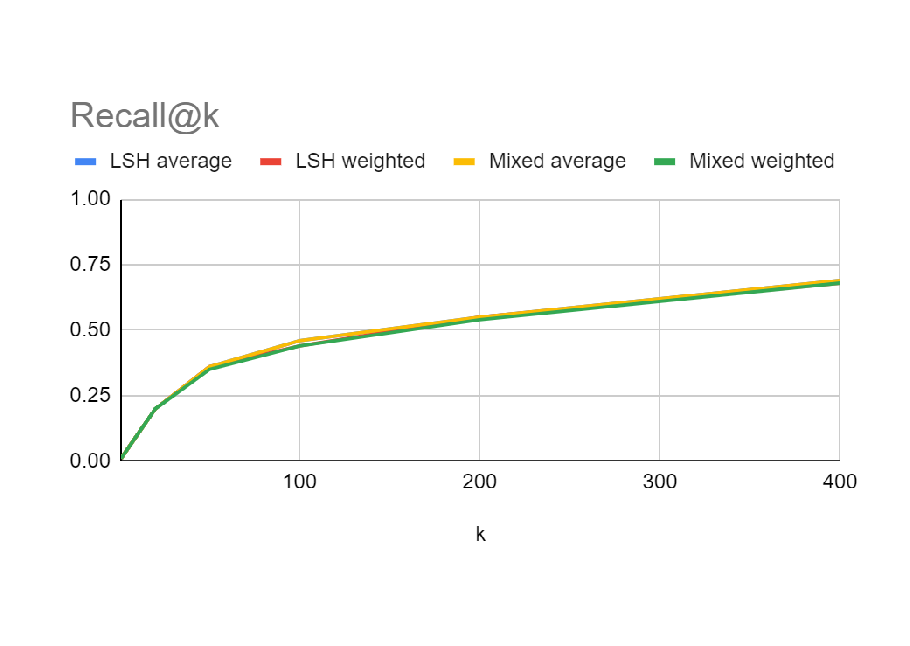
\includegraphics[scale=0.6]{recallAtK.pdf}
    \caption{Recall at various top-k ranking}
    \label{fig:recallAtK}
\end{figure}


\section{Summary Size}\label{summarySizeTest}

To measure the size of the summaries, we divide all of the datasets in 4 sections. The first section contains about 800 columns, the second 3300 columns, the third 5900 columns, and the last 6000 columns. For each sections inserted, we measure the average sketch size (figure \ref{fig:sketchsize}) and the average metadata size (figure \ref{fig:metadatasize}) stored in the database. With each insertion, the average size of the sketches object remain consistent at 6.63kB. This is understandable, as all sketches store the same amount of hash values. Meanwhile, the average size of a metadata object ranges from about 270B to 300B with each iterations. This is due to the fact that the information stored in the metadata is variable: one table name may be very long while other ones are shorter. In total, the metadata and sketches take up about 40MB of storage in the database, meaning the summaries are only 3,55\% of the datasets' original size.

\begin{figure}[ht]
    \centering
    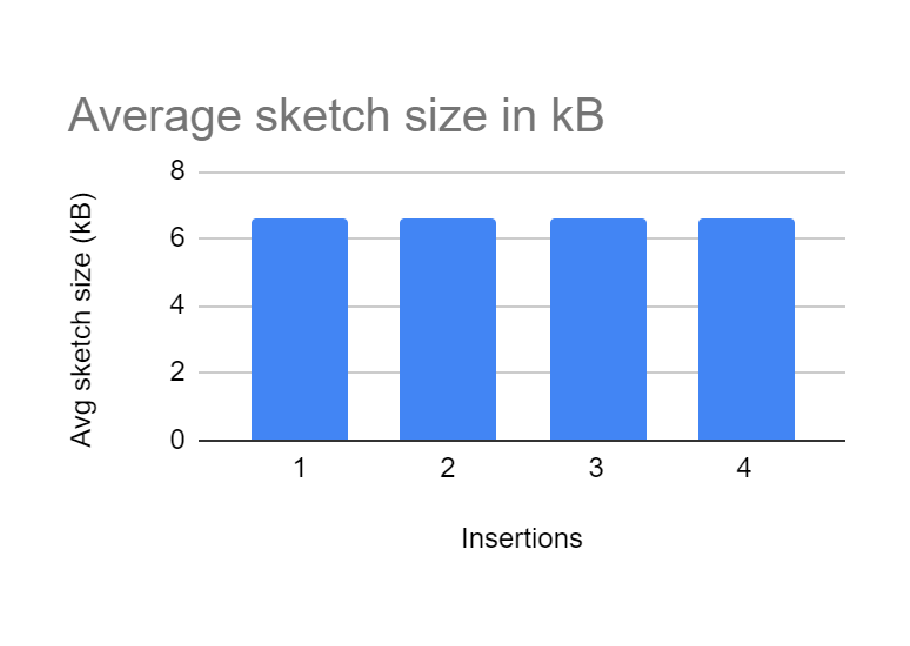
\includegraphics[scale=0.5]{sketchsize.pdf}
    \caption{The average size of the sketches object after each insertions}
    \label{fig:sketchsize}
\end{figure}

\begin{figure}[ht]
    \centering
    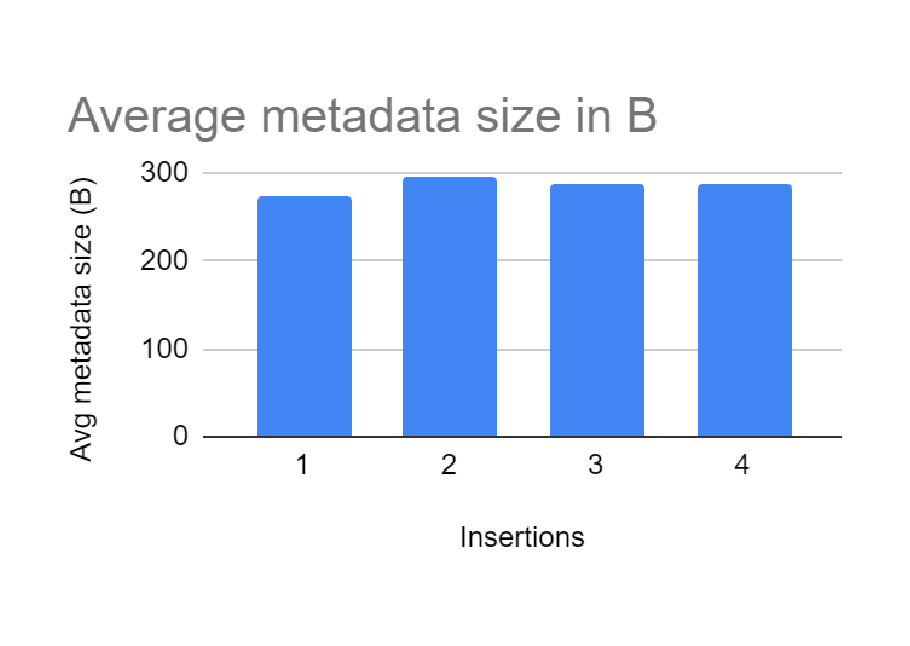
\includegraphics[scale=0.5]{metadatasize.pdf}
    \caption{The average size of the metadata object after each insertions}
    \label{fig:metadatasize}
\end{figure}

\section{Summary Generation Time}

To measure the time it takes to generate summaries, we call the profile() method multiple times on the synthesized Open Data dataset, measuring the time it takes for each types of sketch to be generated, and collect the average runtime. Figure \ref{fig:sketchtime} shows that it took roughly 6 minutes to sketch all columns in the dataset. Most of the time spent were used to generate the values set and the value format, while it took only less than 2 seconds in total for the q-gram sketches of the table name and column name to be generated. Table-wise, it took on average 2 seconds for the profile() method to finish.

\begin{figure}[ht]
    \centering
    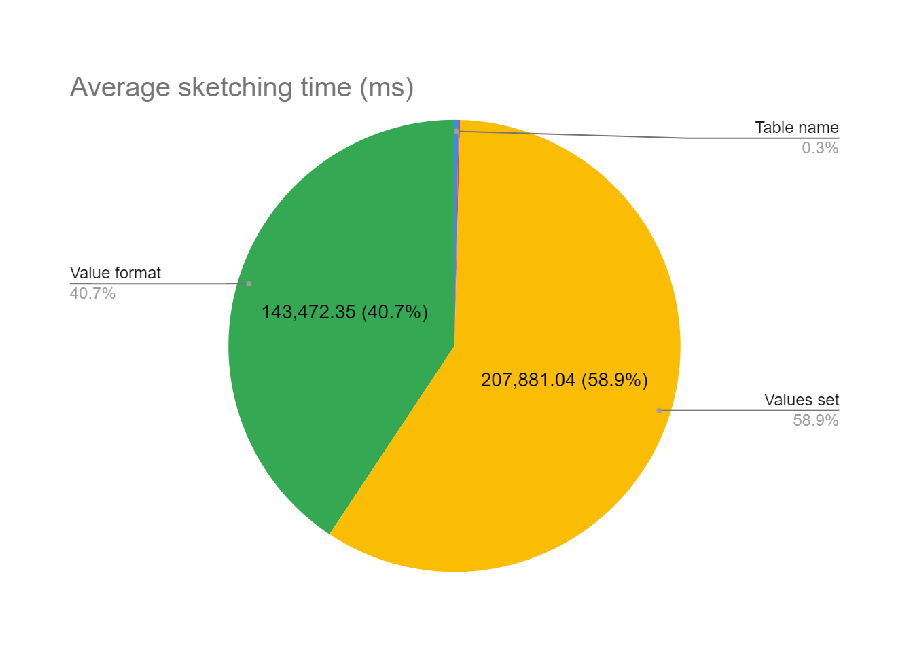
\includegraphics[scale=0.6]{figures/exp1.pdf}
    \caption{Average time taken to sketch the Open Data dataset of 1.1GB}
    \label{fig:sketchtime}
\end{figure}

\section{Effect of in-memory index on startup time}

As mentioned in section \ref{systemArchitecture}, the Lazo's LSH indexes run in main memory. Therefore the sketches need to be loaded from database on startup. We measure the startup time of the system by loading the datasets in 4 sections like in \ref{summarySizeTest}, restarting the server several times for each section loaded, and calculating the average startup time of each iteration. The result is shown in figure \ref{fig:loadIndexTime}, indicating that the startup time grows linearly with the amount of sketches in the database. At the maximum database size containing about 40MB of sketches, the server took roughly 20 seconds to start. As we expect the server to not be restarted often, this time should be negligible.

\begin{figure}[ht]
    \centering
    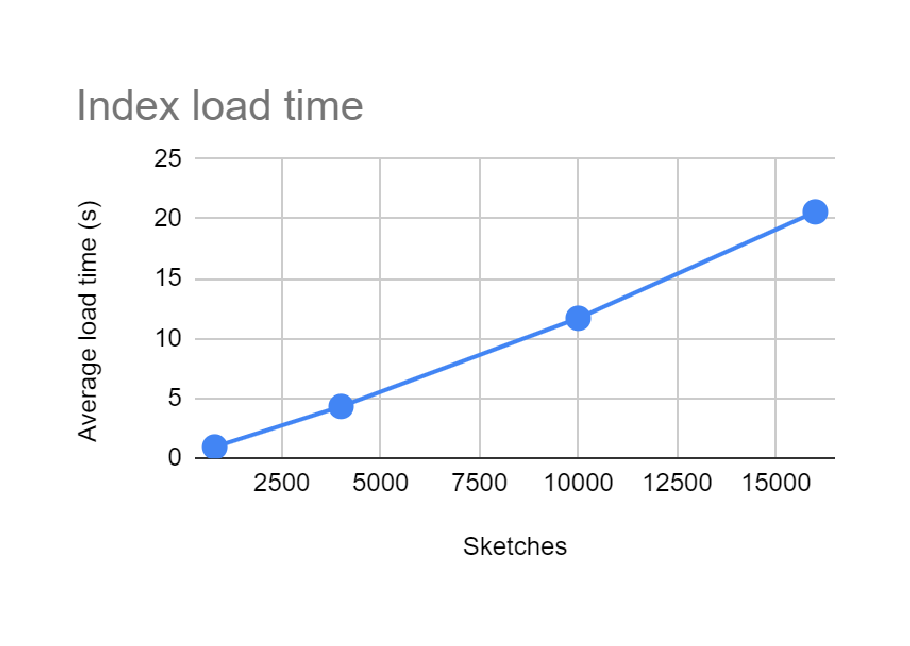
\includegraphics[scale=0.6]{exp2.pdf}
    \caption{Time to startup with increasing amount of sketches}
    \label{fig:loadIndexTime}
\end{figure}

\section{Effect of optimization algorithm}

In this section, we measure the impact of the optimization algorithm \ref{alg:optimization} on the query time. We set up the experiment by first loading all three test datasets into the database, maximizing the amount of candidates that needs to be checked. Then 10 random tables are selected as query, performed at five different query thresholds: 0, 0.2, 0.4, 0.6, 0.8. The similarity measures used are the mixed weighted combinations from \ref{combinedMeasures}. The average runtime at each threshold level is shown in figure \ref{fig:queryThresholdTime}. Without any restriction on the threshold, queries take a long time to calculate. Among our 10 selected queries, there were some that take up to 3 minutes to return. The time reduces on average by 30\% at the 0.4 threshold, and at 0.8 mark, an average query takes only about 10 seconds, which is 6\% of the time taken compared to a 0 threshold. This proves reasonable in practical use cases, as matches with a low similarity score are unlikely to be related anyway.

\begin{figure}[ht]
    \centering
    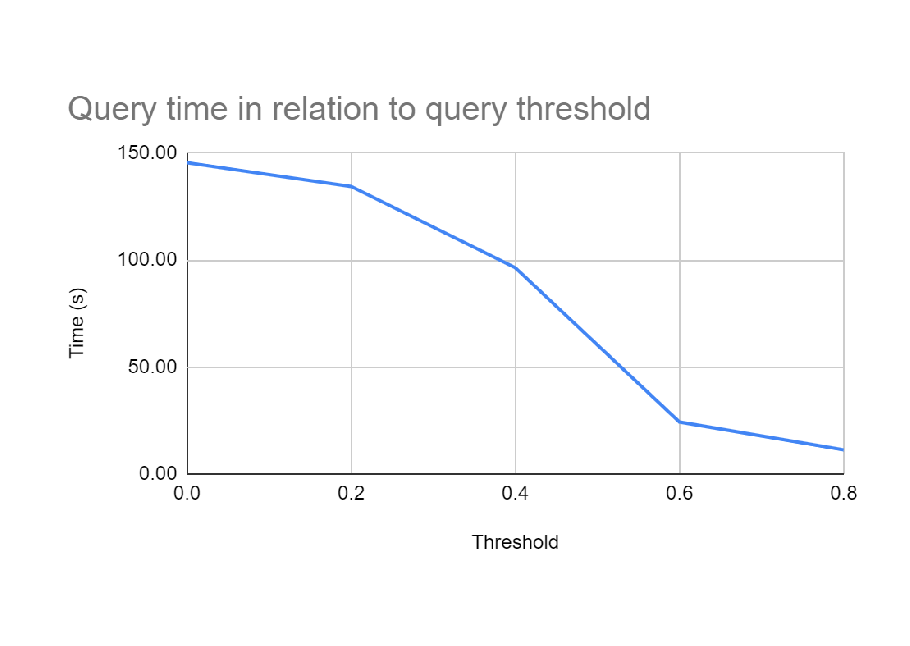
\includegraphics[scale=0.6]{figures/queryThresholdTime.pdf}
    \caption{Query time at various threshold levels}
    \label{fig:queryThresholdTime}
\end{figure}
% !TEX root =  main.tex



\chapter{Conclusion}
\label{chap:conclusion}
\pagestyle{plain}

\section{Limitations}

\section{Future work}



\bibliographystyle{abbrv}
\bibliography{main}

\pagestyle{empty}

\cleardoublepage

\null

\selectlanguage{ngerman}
\subsection*{Eidesstattliche Erklärung}

Ich erkläre hiermit an Eides statt, dass ich die vorliegende Arbeit
selbstständig verfasst und keine anderen als die angegebenen Quellen
und Hilfsmittel verwendet habe. 
\selectlanguage{english}

\subsection*{Statement in Lieu of an Oath }

I hereby confirm that I have written this thesis on my own and that
I have not used any other media or materials than the ones referred
to in this thesis. 

\vspace{2cm}


Kaiserslautern, $\begin{array}[t]{c}
    \text{\_\_\_\_\_\_\_\_\_\_\_\_}\\
    {\scriptscriptstyle \text{Date}}
\end{array}$\hfill{$\begin{array}[t]{c}
    \_\_\_\_\_\_\_\_\_\_\_\_\\
    {\scriptscriptstyle \text{Signature}}
\end{array}$\hfill}

\end{document}
